

%!TEX root = ../thesis.tex
%*******************************************************************************
%****************************** Third Chapter **********************************
%*******************************************************************************
\chapter{Learning from Synthetic Data; Bridging the Domain Gap}\label{chap:cgas}

\def\figref#1{Fig.~\ref{fig:#1}}

% **************************** Define Graphics Path **************************
\ifpdf
    \graphicspath{{Chapter4/Figs/Raster/}{Chapter4/Figs/PDF/}{Chapter4/Figs/}}
\else
    \graphicspath{{Chapter4/Figs/Vector/}{Chapter4/Figs/}}
\fi

% Plan:
% - Introduction - complain about the non-automatic equivalent systems & lack of training data for animals. Impractical to obtain. 
% - Begin with a discussion on systems that use synthetic data for training. Related work should focus on these
% - Discuss methods for generating accurate synthetic data, particularly focus on SURREAL. 
% - Create experiments in which different methods are trained and tested on varying levels of fake data.
% - In-depth explanation of synthetic data creation
% - In-depth explanation of training the joint predictor. Possibly ablate the sampling strategy / architecture. Diagrams etc.
% - Explain why we need to fix with a QP/GA.
% - In depth formulation of the QP and show it works, then explain the GA.
% - Experimental evaluation -- in depth explanation about the data collection exercise etc.
% - Experimental comparison between the two methods
% - In-depth explantion of the SMAL optimizer.
% - Results and comparison to related work
% - Summary 

% Extra experiments: 
% (1) Show that training on synthetic real data doesn't work (e.g. fake textures).
% (2) Use a GAN to generate synthetic data? Why not? Articulated sections didn't work.


\section{Introduction}

This chapter introduces a system for recovering the 3D shape and motion of a wide variety of quadrupedial animals from video. Inspired by techniques from the recent human body and hand tracking literature (most notably SMPLify~\cite{bogo16keep}), the system comprises a machine learning front-end for predicting 2D joint positions followed by an energy minimization stage which fits a detailed 3D model to the image. However, this chapter will discuss a number of key challenges which arise when reconstructing animal subjects compared with humans and methods to overcome them.

\subsection{Limited animal training data}
For human tracking, hand labelled sequences of 2D segmentations and joint positions have been collected from a wide variety of sources~\cite{andriluka14cvpr,lin2014microsoft,johnson2010clustered}. Of these two classes of labelling, animal {\em segmentation} data is available in datasets such as MSCOCO~\cite{lin2014microsoft}, PASCAL VOC~\cite{everingham2010pascal} and DAVIS~\cite{Perazzi2016}.  However this data is considerably sparser than human data, and must be ``shared'' across species, meaning the number of examples for a given animal shape class is considerably fewer than is available for an equivalent variation in human shape.  While segmentation data can be supplied by non-specialist human labellers, it is more difficult to obtain {\em joint position} data.  Some joints are easy to label, such as ``tip of snout'', but others such as the analogue of ``right elbow'' require training of the operator to correctly identify across species. In the case of SMPLify, the network is trained on large-scale human keypoint datasets, including MPII~\cite{andriluka14cvpr} (approx. 40,000 people) and the Leeds Sport Dataset~\cite{johnson2010clustered}. Unfortunately, there is no keypoint dataset for animals that cover even a small fraction of the quadruped types that we aim to reconstruct. 

Of greater concern however, is 3D skeleton data.  For humans, motion capture (mocap) can be used to obtain long sequences of skeleton parameters (joint positions and angles) from a wide variety of motions and activities. For animal tracking, this is considerably harder: animals behave differently on treadmills than in their quotidian environments, and although some animals such as horses and dogs have been coaxed into motion capture studios~\cite{wilhelm2015furyexplorer}, it remains impractical to consider mocap for a family of tigers at play.

These dataset challenges have, at least in part, resulted in the lack of \emph{automatic} approaches for 3D animal reconstruction. Precisely, prior to the design of the system discussed in this chapter, 3D animal reconstruction techniques relied on at least one of manually provided silhouettes, keypoint locations or limb tracks. The techniques are summarized in \Cref{tab:animal-annot-tab} and discussed in depth in \Cref{chap:relwork}. 



% \newcommand{\awfhang}[1]{
%     \begin{minipage}[t]{\textwidth}% Top-hanging minipage, will align on
%                                    % bottom of first line
%     \begin{tabbing} % tabbing so that minipage shrinks to fit
%     \\[-\baselineskip] % Make first line zero-height
%     #1 % Include user's text
%     \end{tabbing}
%     \end{minipage}} % can't allow } onto next line, as {WIDEBOX}~x will not tie.
    
    \newcolumntype{L}[1]{>{\RaggedRight\hspace{0pt}}p{#1}}
    \newcolumntype{R}[1]{>{\RaggedLeft\hspace{0pt}}p{#1}}
    
    \begin{table}[t!]
    {\sffamily
    \scriptsize
    \def\hd#1{\awfhang{#1}}
    \begin{tabular}{@{}L{20mm}%Paper
    L{10mm}%Year
    |L{12mm}%Class
    L{15mm}%Train
    |L{15mm}%Template
    L{17mm}%Video
    L{17mm}%Test
    |L{9mm}%Model
    L{5mm}%Size
    @{}}
    \hd{Paper}%
    &\hd{Release\\Year}%
    &\hd{Animal\\Class}%
    &\hd{Training\\requirements}%
    &\hd{Template\\Model}%
    &\hd{Video\\required}%
    &\hd{Test Time\\Annotation}%
    &\hd{Model\\Fitting}%
    &\hd{Test\\Size}%
    \\\hline
    %%%%%%%%%%%%%%%%%%%%%%
    What Shape are Dolphins~\cite{cashman2013shape}
    & 2013
    & Dolphins, Pigeons 
    & Not trained
    & Dolphin Template
    & 25 frames / category & J2, S2 & Yes & 25
    \\\hline
    %%%%%%%%%%%%%%%%%%%%%%
    Animated 3D Creatures~\cite{reinert2016animatedsketching}
    & 2016
    & MLQ
    & Not trained
    & Generalized Cylinders
    & Yes & J2, S2 & Yes & 15
    \\\hline
    %%%%%%%%%%%%%%%%%%%%%%
    3D Menagerie (SMAL)~\cite{zuffi2017menagerie}       
    & 2017         
    & MLQ 
    & Not trained
    & SMAL
    & No & J2, S2 & Yes & 48 
    \\\hline
    %%%%%%%%%%%%%%%%%%%%%%
    Category Specific Mesh Reconstructions~\cite{kanazawa2018birds}
    & 2018
    & Birds
    & J2, S2
    & Bird convex hull
    & No & None & No & 2850          
    \\\hline
    %%%%%%%%%%%%%%%%%%%%%%
    Lions, Tigers and Bears (SMALR)~\cite{zuffi_lions} 
    & 2018
    & MLQ
    & Not trained
    & SMAL
    & 3-7 frames / animal & J2, S2 & Yes & 14
    \\\hline
    %%%%%%%%%%%%%%%%%%%%%%
    This paper
    & 2018
    & MLQ
    & Not trained
    & SMAL
    & Yes & S2 (for best results shown) & Yes & 9
    \\\hline 
    %%%%%%%%%%%%%%%%%%%%%%
    Who Left the Dogs Out?
    & 2018
    & Dogs  % 2D Joints, Silhouettes, 3D Template, 3D Priors
    & J2, S2, T3, P3
    & SMAL
    & No & None & No & 1703
    \\\hline
    %%%%%%%%%%%%%%%%%%%%%%
    3D-Safari~\cite{Zuffi19Safari}        
    & 2019
    & Zebras, horses
    % 3D models (albeit synthetic), 2D Joints,  Silhouettes,  3D Priors
    & M3 (albeit synthetic), J2, S2, P3
    & SMAL
    & 3-7 frames / animal & None & Yes & 200
    \\\hline
    %%%%%%%%%%%%%%%%%%%%%%
    U-CMR~\cite{Zuffi19Safari}        
    & 2020
    & Birds
    % 3D models (albeit synthetic), 2D Joints,  Silhouettes,  3D Priors
    & M3 (albeit synthetic), J2, S2, P3
    & Bird convex hull
    & 3-7 frames / animal & None & Yes & 200
    \\\hline
    \end{tabular}
    }
    \caption{Literature summary: Analysis of required input annotations.
    MLQ: Medium-to-large quadrupeds. J2: 2D Joints. S2: 2D Silhouettes. T3: 3D Template. P3: 3D Priors. M3: 3D Model.}
    \label{tab:animal-annot-tab}
    % \vspace{-8mm}
    \end{table}
    
    


\subsection{Synthetic image generation}

In the absence of real-world motion capture data, the recent publication of the Skinned Multi-Animal Linear (SMAL) model~\cite{zuffi2017menagerie} offers a method for \emph{synthetic} data generation. Analogous in design to the popular SMPL~\cite{loper15smpl} parametric human model, SMAL can generate a wide range of quadruped species. As discussed in \Cref{chap:relwork}, SMAL overcomes the lack of 3D animal training data by instead learning from 41 scans of toy figurines. This results in SMAL being of considerably lower fidelity than the SMPL, which was constructed from 1786 3D human scans. However, the model's PCA shape space offers a mechanism for sampling potentially infinite quadruped animals of satisfactory realism which can form a valuable training dataset.

% comes without surface texture maps. 
The use of synthetic images to train 3D reconstruction systems has been attempted in recent computer vision literature. The general approach is to capture training images by capturing multiple images of a representative 3D model (or scene) by randomly sampling camera and environmental parameters. A machine learning model is then trained on this dataset $D_{synth}$ of synthetic images and later tested on a dataset $D_{real}$ of real-world examples. This procedure offers an important practical advantage; the training images can be automatically generated with correponding annotations. Depending on the task, this can overcome a lengthy and complex process of sourcing manual annotations from users. However, designing a data pipeline which can generate synthetic images with sufficient realism to be representative of real test images $D_{real}$ is challenging. A common pitfall of such approaches is the tendancy to train machine learning models that perform well on unseen synthetic images but poorly on real world examples. This phenomenon is often caused by systematic differences between the $D_{synth}$ and $D_{real}$, resulting in the model becoming overreliant on features present only in $D_{synth}$ or unfamiliar with features present only in $D_{real}$. The differences between datasets is often described as the \emph{domain gap} which must be bridged in order to achieve a successful predictor. 

%Review paper: https://arxiv.org/pdf/1909.11512.pdf?fbclid=IwAR2FuZvNAlIGuyh2wtVEmj_rLzjaJvCjMNWP_svBqhMtnXcEX-NV9z8rR7g
Fortunately, there are a number of options for tackling this problem. A popular strategy is to ensure the generation pipeline is of extremely high quality. SURREAL\lazycite{SURREAL}{SURREAL} is a method which learns from synthetic human images rendered using the popular SMPL~\cite{loper15smpl} parametric model. In this work, the authors go to significant effort to source realistic UV texture maps for SMPL and apply a high quality rendering engine complete with a lighting and reflectance model to generate their training images. A similar approach is followed by SMALST \lazycite{SMALST}{SMALST}, who follow a multi-view optimization pipeline to construct a synthetic zebra training dataset complete with realistic textures. Related also are autonomous driving systems that train (or pre-train) on synthetic `virtual worlds' \lazycite{https://arxiv.org/pdf/1605.06457.pdf?fbclid=IwAR0RtcIEKYgghwD5uo_TSwesiD2XuhqaQtuoTaQe2omp-QCdzJv4O3PjBjU}{Virtual Worlds}. An alternative option is to process the test image dataset to find a representation which is easier to synthesise. For 3D human skeleton prediction, Shotton et al.~\cite{shotton-kinect} synthetise a set of depth images used to train a keypoint regressor. An unfortunate byproduct of this training style however is that it necessitates a depth sensor at test time. 

%Related also is the work of \lazycite{GTA-Cars}{GTA-Cars} who use a images rendered from a popular video game engine to teach an automous agent to drive with reinforcement learning. 
%Another category of approaches are found in optical flow. Optical flow is an example of a dense point correspondence task: given two frames $I_{i}, I_{i+1}$ a model should predict a \emph{flow field} $f: \RR{H}{W} \mapsto \RR{H}{W}$. Of course, for this task the most important learning signal is obtained through observing object and camera \emph{motion}. For this reason, multiple models are trained using the FlyingChairs dataset: since natural scenes are complex to generate, models can just learn from flow directly. % Tidy up this argument

A significant advance has been made recently with the introduction of generative adversarial networks (GANs). This is a worthy direction and has been considered fully in \Cref{chap:summary} of this thesis. 


of this is that there should be an analoug% TODO: Justify why GANs are a bad idea...
% Mode collapse
% With GANs, there should be an anology between shapes in the real and synthetic set. However, it's difficult to render synthetic shapes which match shapes in an unlabelled test dataset. 

The system presented in this section adopts an alternative (and much simpler) approach for synthetic image generation. The idea builds on the realisation that a 2D silhouette image encodes a significant amount of the object's shape features, and by virtue of being textureless and having no background detail is much simpler to synthesise. As previously discussed, there are also a great number of `off-the-shelf' image segmentation engines which can produce accurate animal silhouettes of a high quality. 

The joint candidate predictor is trained on synthetically generated silhouette images, and at test time, deep learning methods or standard video segmentation tools are used to extract silhouettes from real data. The system is tested on animal videos from several species, and shows accurate reconstructions of 3D shape and pose.


\subsection{Handling silhouette ambiguity}

An unfortunate drawback of using silhouette images (for example, when compared to RGB or depth counterparts) is that missing interior contours leads to a source of reconstruction ambiguity. An example of this is shown in Figure 6 in which two distinct 3D reconstructions are shown to yield similar 2D silhouette reprojections. Clearly, a naive joint predictor which regreses a single set of 2D coordinates from an input silhouette would perform suboptimally, since the silhouette alone contains insufficient information to resolve such cases. 

However, the fact that the system is designed to accept a video sequence as input (rather than a single frame) provides additional information which can be used to resolve per-frame ambiguities. This section describes a method for incoporating temporal knowledge in order to obtain a reliable set of predicted 2D joint coordinates that later form the basis for the 3D model fitting stage. The key insight is to modify a standard joint heatmap predictor~\lazycite{hourglassnet} {hourglassnet} in order to encourage multi-modal outputs, both when trained on synthetic data and later tested on real world frames. A novel discrete optimization stage is then used to recover the skeleton trajectory of maximal likelihood from the sequence of multi-modal predictions. This section will explore two methods for achieving this: the first frames the problem as a quadratic program and the later provides achieves a significant efficiency improvement by using a genetic algorithm. 


%The system comprises a machine learning front-end which predicts candidate 2D joint positions, a discrete optimization which finds kinematically plausible joint correspondences, and an energy minimization stage which fits a detailed 3D model to the image. 


% The core methodologies are inspired by techniques from the recent human body and hand tracking literature, combining machine learning and 3D model fitting. A discriminative front-end uses a deep hourglass network to identify candidate 2D joint positions. These joint positions are then linked into coherent skeletons by solving an optimal joint assignment problem, and the resulting skeletons create an initial estimate for a generative model-fitting back-end to yield detailed shape and pose for each frame of the video.  

% For human tracking, hand labelled sequences of 2D segmentations and joint positions have been collected from a wide variety of sources~\cite{andriluka14cvpr,lin2014microsoft,johnson2010clustered}. Of these two classes of labelling, animal {\em segmentation} data is available in datasets such as MSCOCO~\cite{lin2014microsoft}, PASCAL VOC~\cite{everingham2010pascal} and DAVIS~\cite{Perazzi2016}.  However this data is considerably sparser than human data, and must be ``shared'' across species, meaning the number of examples for a given animal shape class is considerably fewer than is available for an equivalent variation in human shape.  While segmentation data can be supplied by non-specialist human labellers, it is more difficult to obtain {\em joint position} data.  Some joints are easy to label, such as ``tip of snout'', but others such as the analogue of ``right elbow'' require training of the operator to correctly identify across species.

% Of more concern however, is 3D skeleton data.  For humans, motion capture (mocap) can be used to obtain long sequences of skeleton parameters (joint positions and angles) from a wide variety of motions and activities.
% For animal tracking, this is considerably harder: animals behave differently on treadmills than in their quotidian environments, and although some animals such as horses and dogs have been coaxed into motion capture studios~\cite{wilhelm2015furyexplorer}, it remains impractical to consider mocap for a family of tigers at play.

\subsection{Contributions}


\begin{figure}[t]
\def\p#1#2{\parbox{0.32\linewidth}{
\labelledpic{\includegraphics[trim={4cm 7cm 4cm 7cm},clip,width=\linewidth]{sys_overview_pred_2/#2.jpg}}
{\scriptsize #1}}}
\def\ps#1#2{\parbox{0.32\linewidth}{
\labelledpic{\includegraphics[trim={0cm 2cm 0cm 2cm},clip,width=\linewidth]{sys_overview_pred_2/#2.jpg}}
{\scriptsize #1}}}
\p a{rgb}             \p b{target}         \p c{heatmap}
\p d{skeleton_sil}    \p e{00048_overlay}  \ps f{00048_alternative}
\caption{{\bf System overview}: input video (a) is automatically processed using DeepLabv3+~\cite{deeplabv3plus} to produce silhouettes (b), from which 2D joint predictions are regressed in the form of heatmaps (c).  Optimal joint assignment (OJA) finds kinematically coherent 2D-to-3D correspondences~(d), 
which initialize a 3D shape model, optimized to match the silhouette~(e). 
Alternative view shown in (f).
}
\label{fig:overview}
\end{figure}

Taking into account the above constraints, this work applies a novel strategy to animal tracking, which assumes a machine-learning approach to extraction of animal silhouettes from video, and then fits a parameterized 3D model to silhouette sequences.  The system exhibits the following contributions:
\begin{itemize}
\item A machine-learned mapping from silhouette data of a large class of quadru\-peds to generic 2D joint positions.
\item A novel optimal joint assigment (OJA) algorithm extending the bipartite matching of Cao {\em et al.}~\cite{cao2017realtime} in two ways, one which can be cast as a quadratic program (QP), and an extension optimized using a genetic algorithm (GA).
\item A procedure for optimization of a 3D deformable model to fit 2D silhouette data and 2D joint positions, while encouraging temporally coherent outputs.
\item We introduce a new benchmark animal dataset of joint annotations (BADJA) which contains sparse keypoint labels and silhouette segmentations for eleven animal video sequences. 
Previous work in 3D animal reconstruction has relied on bespoke hand-clicked keypoints~\cite{zuffi2017menagerie,zuffi_lions} and little quantitative evaluation of performance could be given.
The sequences exhibit a range of animals, are selected to capture a variety of animal movement and include some challenging visual scenarios such as occlusion and motion blur.
\end{itemize}

The system is outlined in \figref{overview}.  The remainder of the paper provides a detailed description of system components.  Joint accuracy results at multiple stages of the pipeline are reported on the new BADJA dataset, which contains ground truths for real animal subjects. Experiments are also conducted on synthetic animal videos to produce 3D joint accuracy statistics and full mesh comparisons. A qualitative comparison is given to recent work~\cite{zuffi2017menagerie} on the related single-frame 3D shape and pose recovery problem. The paper concludes with an assessment of strengths and limitations of the work.

% \subsection{Related Work}
% In this section, we will discuss work specifically related to this paper. The broad 

% \subsubsection{Non-automatic approaches for 3D reconstruction of articulated subjects}

% Much of this is handled in the previous section, but could be briefly recapped. Point out that we want an AUTOMATIC technique that can rapidly apply across different quadruped types.

% \subsubsection{Automatic approaches for 3D reconstruction of articulated subjects}

% The SMPLify approach is comprises of two stages, means of achieving 3D human reconstruction. an automatic To train such a system, we may look towards the SMPLify technique employed for 3D human mesh recovery


% \subsubsection{Learning from synthetic data}

% SURREAL dataset for humans. 

% \subsubsection{Cleaning up predictions}

% Talk about pictorial structure models. Could be integrated later.

% \section{Design discussion for an automatic quadruped 3D reconstruction}
% \def\seq#1#2#3#4{\left[{#1_{#2}}\right]_{#2=#3}^{#4}}

% The test-time problem to be solved is to take a sequence of input images and for each image, output the shape, pose and position parameters describing the animal's motion.

% To train such a system, we start by considering the suitability of the SMPLify~\cite{bogo16keep} method (discussed above) which describes a two-stage approach for automatic 3D human reconstruction. However, the approach has particular design requirements that prevents trivial extension to reconstructing quadrupeds. 

% \subsection{Keypoint training data for joint predictor}

% Firstly, the preliminary stage of the approach is based on the DeepCut joint predictor, a convolutional neural network that takes an input an image and predicts a set of semantically meaningful keypoints. In the case of SMPLify, the network is trained on large-scale human keypoint datasets, including MPII~\cite{andriluka14cvpr} (approx. 40,000 people) and the Leeds Sport Dataset~\cite{johnson2010clustered}. As previously discussed, there are no keypoint datasets for animals that cover even a small fraction of the quadruped types that we aim to reconstruct. 

% With no real-world data to use for training the keypoint predictor, we can turn instead to a novel approach that instead relies on synthetic (or fake) data for training. 


% \subsection{Data driven shape and pose priors}

% Of course, we also don't have any shape or pose priors.


\section{Preliminaries}

\subsection{Deformable 3D quadruped model}

This section provides a formal definition for the deformable 3D model that is used to generate synthetic training data and in the model fitting stage to obtain the final mesh. Our system assumes a deformable 3D model such as SMAL~\cite{zuffi2017menagerie} which parametrizes a 3D mesh as a function of {\em pose} parameters~$\pose \in \R\npose$ (e.g.\ joint angles) and {\em shape} parameters~$\shape \in \R\nshape$. 
As discussed in \Cref{chap:relwork}, a 3D mesh is an array of vertices $\verts \in \RR 3\nverts$ (the vertices are columns of a $3 \times \nverts$ matrix) and a set of triangles represented as integer triples $(i,j,k)$, which are indices into the vertex array.
A deformable model such as SMAL may be viewed as supplying a set of triangles, and a function
\begin{equation}
\verts(\pose, \shape) : \R \npose \times \R \nshape \mapsto \RR 3 \nverts
\end{equation}
which generates the 3D model for a given pose and shape.
The mesh topology (i.e.~the triangle vertex indices) is provided by the deformable model, and is the same for all shapes and poses we consider, so in the sequel a mesh will be defined only by the 3D positions of its vertices.

In any given image, the model's 3D {\em position} (i.e.\ translation and orientation) is also unknown, and will be represented by a parametrization $\posn$ which may be for example translation as a 3-vector and rotation in axis angle form. Application of such a transformation to a $3\times\nverts$ matrix will be denoted by $*$, so that 
\begin{equation}
\posn * \verts(\pose, \shape)
\end{equation}
represents a 3D model of given pose and shape transformed to its 3D position.

It is also necessary to define a model's {\em joints}.  These appear naturally in models with an explicit skeleton, but more generally they can be defined as some function mapping from the model parameters to an array of 3D points analogous to the vertex transformation above. Note that even in the case of rigged models, this provides a mechanism to add additional joints beyond the ones required to drive model deformation. In any case, joints are defined by post-multiplying by a $\nverts \times \njoints$ matrix $\jointselect$.  The $j^{\text{th}}$ column of~$\jointselect$ defines the 3D position of joint~$j$ as a linear combination of the vertices (this is quite general, as $\verts$ may include vertices not mentioned in the triangulation).  

\subsection{Camera model, joint reprojection and silhouette rendering}
For both synthetic image generation and the later model fitting stage, it is necessary to be able to \emph{render} the 3D model. A general camera model is described by a function $\proj: \R{3} \mapsto \R{2}$.  This function incorporates details of the camera intrinsics such as focal length, which are assumed known.  
Thus 
\begin{equation} \label{eq:project_joints}
\kappa(\posn, \pose, \shape) := \proj(\posn * \verts(\pose, \shape) \jointselect)
\end{equation}
is the $2\times \njoints$ matrix whose columns are 2D joint locations corresponding to a 3D model specified by (position, pose, shape) parameters $(\posn, \pose, \shape)$.

The model is also assumed to be supplied with a rendering function $R$ which takes a vertex array in camera coordinates, and generates a 2D binary image of the model silhouette.  That is,
\begin{equation} \label{eq:render_sil}
R\bigl(\posn * \verts(\pose, \shape)\bigr) \in \mathbb{B}^{W\times H}
\end{equation}
for an image resolution of $W \times H$.  In order to allow derivatives to be propagated through $R$ (essential for the silhouette term in the model fitting stage), the \emph{differentiable renderer} of Loper et al.~\cite{loper2014opendr} is used. Please see the relevant section in \Cref{chap:relwork} for further details.

\subsection{System overview}

The test-time problem to be solved is to take a sequence of input images
\[
\mathcal{I} = \seq{I}{t}{1}{T}
\]
which are segmented to the silhouette of a single animal (i.e.~a video with multiple animals is segmented multiple times), producing a sequence of binary silhouette images 
\[
\mathcal{S} = \seq{S}{t}{1}{T}.
\]

The computational task is to output for each input image the shape, pose, and position parameters describing the animal's motion. Inspired by recent work in human 3D reconstruction, this objective can be broken down into a multiple stage pipeline. 

The core components are as follows:

\begin{enumerate}
    \item The discriminative front-end extracts silhouettes from video, and then uses the silhouettes to predict multi-modal heatmaps, from which 2D joint positions are obtained with multiple candidates per joint. 
    \item Optimal joint assignment (OJA) corrects confused or missing skeletal predictions by finding an optimal assignment of joints from a set of network-predicted proposals. 
    \item Generative deformable 3D model is fitted to the silhouettes and joint candidates as an energy minimization process.
\end{enumerate}

These stages are described in detail over the following three sections.


\section{Predicting 2D joint candidate locations}

% Explain hourglass network, it's structure and why it's good.
The goal of the first stage is to take, for each video frame, an image reperesenting the animal and to output a $W \times H \times \njoints$ tensor of heatmaps. To achieve this, we train the stacked hourlgass network~\cite{newell2016stacked} of Newell et al. to a large dataset of synthetically generated quadruped images. 

\subsection{Generating synthetic quadruped images}

In order to render a synthetic quadruped image, a set of pose $\pose$, shape $\shape$ and position $\posn$ parameters are required. With these parameters, a (textureless) training image can be generated by applying \Cref{eq:render_sil} and corresponding ground truth 2D joints locations can be generated via \Cref{eq:project_joints}. What remains is to ensure a model trained on the synthetic images generalizes to the real-world test images. To achieve this, it is important that the training dataset captures the modes of variation by appropriately sampling the model parameters. 

\subsubsection{Sampling shape and pose parameters}

Given that the real-world test images exhibit multiple quadruped species, a primary mode of variation is the animal's \emph{shape} characterisitics. Naively, generating a dataset large enough to capture possible test animal shapes would be a challenging task, since it would require access to multiple real or artist-generated 3D scans. Fortunately, the SMAL model defines a linear shape space which allows repeated sampling of different (and realistic) quadruped shapes. Of course, having been built from only toy figurines, the variation is still somewhat limited, but as the later experimental section will show, the model is fit for purpose. Synthetic shape parameters $\shape$ are obtained by sampling from a Gaussian prior:

\begin{equation}\label{eq:sampling_shape}
X = Y
\end{equation}

Another mode of variation in test images is the various animal limb positions. These can again be synthetised by sampling from a gaussian prior constructed from a dataset of animal poses. Since no such dataset exists for real animals, a prior is instead built from a small set of artist-generated poses, originally provided by the SMAL model authors. The sampling strategy is therefore given by:


\begin{equation}\label{eq:sampling_pose}
    X = y
\end{equation}


\subsubsection{Sampling position (camera) parameters}

The random camera positions are generated as follows: the orientation of the camera relative to the animal is uniform in the range $[0, 2\pi]$, the distance from the animal is uniform in the range 1 to 20 meters and the camera height is in the range $[0,\frac{\pi}{2}]$. This smaller range is chosen to restrict unusual camera elevation. Finally, the camera ``look" vector is towards a point uniformly in a 1m cube around the animal's center, and the ``up" vector is Gaussian around the model Y axis.

\subsubsection{What about textures and backgrounds?} 

At this point, the synthetic test images have plausible shape, pose and positional parameters but are lacking in realistic texture. Furthermore, it is not clear how to render plausible background scenes, nor how to convincingly place the 3D animal in such a scene. This challenge allows for a primary contribution of this work: using the silhouette domain as a representation much easier to synthetise (since surface texture maps and background textures are lost) and can be obtained from real-world test images. Another important characteristic of the mapping between real-world images and silhouette counterparts is that the shape and pose information is mostly preserved, apart from a few ambiguities (e.g. limb ordering due to lacking interior contours). 

To summarise, training data comprises $(S, \kappa)$ pairs, that is pairs of binary silhouette images, and the corresponding 2D joint locations as a $2\times J$ matrix. See an example in   To generate each image, a random shape vector $\shape$, pose parameters $\pose$ and camera position $\posn$ are drawn, and used to render a silhouette $R\bigl(\posn * \verts(\pose, \shape)\bigr)$ and 2D joint locations $\kappa(\posn,\pose,\shape)$.


% The corresponding 2D joint positions, represented as a $2\times \njoints$ matrix are given, as above, by
% \[
%     \kappa(\posn, \pose, \shape) := \proj(\posn * \verts(\pose, \shape) \jointselect)
% \]

\subsection{Prediction of 2D joint locations using multimodal heatmaps}

% explain that the quality of the joint prediction, while good still leaves unsatisfactory predictions which can cause problems to the later energy minimization steps. To overcome this, 


A pose estimation network can now be trained on a dataset of binary silhouette images $S$ with corresponding 2D joint locations $\kappa(\posn,\pose,\shape)$. The core network architecture used for this task is the stacked hourglass network~\cite{newell2016stacked} of Newell et al., with an adaptation to produce multi-modal outputs. The stacked hourglass network is now briefly described:

\subsubsection{Stacked hourglass network}

A stacked hourglass network is a convolutional neural network specifically designed for the task of pose estimation. Hourglass allows inference to take place across multiple scales; an important advantage allowing the network to reason about global information (such as the full body) and local information (such as face features). This is achieved using a repeated bottom-up, top-down modules which each produce a $W \times H \times \njoints$ heatmap tensor. Supervision is applied to each of these heatmaps, which are then passed to ths subsequent block, allowing high level features to be reevaluated for higher order spatial relationships (generally only present at low resolutions). The network's architecture can be seen in detail in Figure XXX. Hourglass uses a mean squared error loss against a ground truth heatmap tensor, which is applied to the network's final output and all intermediatary hetamaps. Therefore, ground truth joint coordinates $\kappa(\posn,\pose,\shape)$ must first be encoded into a $W \times H \times \njoints$ tensor of heatmaps. The original authors find that the network has better convergence properties if the ground truth heatmaps are blurred slightly, since a gradient is then provided to predicted ``near misses''. This is achieved by blurring ground truth heatmaps with a Gaussian kernel of radius $\sigma$. The final 2D joint positions are then obtained using non-maximum suppression on the output heatmaps

\begin{equation}\label{eq:non-max-suppression}
    A = B    
\end{equation}

\subsubsection{Adaptations for training on synthetic data}

This setup is mostly suitable for training on synthetic quadruped data, subject to a couple of adaptations. Firstly, the silhouette training images differ considerably in appearance to the RGB images used by the original Hourglass authors. A common difficulty for training pose estimation networks on full RGB images is in trying to distinguish between objects and the background class. With binary silhouette images, this distinction is made trivial as background and foreground are assigned values $0$ or $1$ respectively. Unfortunately, this causes a problem when naively training HourglassNet on the generated synthetic images as the network can greatly minimize the loss by simply predicting `background' for every image pixel (since background pixels tend to outnumber foreground pixels). The fact that `background' is a much simpler class to predict than the other joint classes causes a training instability which is challenging to overcome by adjusting the learning rate. Instead, the loss function is replaced with a \emph{weighted} version of the mean squared error loss. This modification encourages the network to devote it's attention to all classes equally. The precise formulation for this is given as follows:

\begin{equation}\label{eq:weighted-mse}
    A = B
\end{equation}


\subsubsection{Adapting stacked hourglass network for multi-output learning}

As detailed in the later experimental section, the network trained using this process generalizes well from synthetic to real images due to the use of the silhouette, and produces accurate predictions for most joints. However, the predictor performs poorly on some joints due to ambiguities which result from the lack of interior contours in the silhouette input data. These missing details cause often result in confusion between joint ``aliases'': left and right or front and back legs.  When these predictions are wrong and are represented by high confidence heatmap regions, little probability mass is assigned to the area around the correct leg, meaning no available proposal is present after non-maximal suppression.

This is handled with a further technical contribution; handling the prediction uncertainty by adapting the stacked hourglass network to produce multiple outputs. This is achieved by explicitly training the network to assign some probability mass to the ``aliased'' joints. For each joint, a list of potential aliases are defined as weights $\lambda_{j,j'}$ and linearly blend the unimodal heatmaps $G$ to give the final training heatmap $H$:

\begin{equation}
    H_{j}(p) = \sum_{j'} \lambda_{j,j'} G(p; \kappa_{j'}, \sigma)
\end{equation}

For non-aliased joints $j$ (all but the legs), $\lambda_{j,j} = 1$ and $\lambda_{j,j'} = 0$, yielding the unimodal maps. For aliased joints, the joint is assigned a weight $\lambda_{j,j} = 0.75$ and aliases are assigned a weight $\lambda_{j,j'} = 0.25$. This ratio is shown to ensure opposite legs have sufficient probability mass to pass through a modest non-maximal suppression threshold without overly biasing the skeleton with maximal predicted confidence. An example of a heatmap predicted by a network trained on multimodal training samples is illustrated in \figref{single_multi}. Note that the construction of at most bi-modal ground truth heatmaps sets a practical constraint on the number of output modes. In other words, the loss is minimized if the network produces one output mode for non-aliased joints and two output modes for aliased joints. 

% % Please add the following required packages to your document preamble:
% \usepackage{booktabs}
\begin{table}[]
    \begin{tabular}{@{}lllll@{}}
    \toprule
    Joint ID & Joint Name                    & Weight & Alias                         & Alias Weight \\ \midrule
    0        & Left front leg: paw           & 0.75   & Right front leg: paw          & 0.25         \\
    1        & Left front leg: middle joint  & 0.75   & Right front leg: middle joint & 0.25         \\
    2        & Left front leg: top           & 0.75   & Right front leg: top          & 0.25         \\
    3        & Left rear leg: paw            & 0.75   & Right rear leg: paw           & 0.25         \\
    4        & Left rear leg: middle joint   & 0.75   & Right rear leg: middle joint  & 0.25         \\
    5        & Left rear leg: top            & 0.75   & Right rear leg: top           & 0.25         \\
    6        & Right front leg: paw          & 0.75   & Left front leg: paw           & 0.25         \\
    7        & Right front leg: middle joint & 0.75   & Left front leg: middle joint  & 0.25         \\
    8        & Right front leg: top          & 0.75   & Left front leg: top           & 0.25         \\
    9        & Right rear leg: paw           & 0.75   & Left rear leg: paw            & 0.25         \\
    10       & Right rear leg: middle joint  & 0.75   & Left rear leg: middle joint   & 0.25         \\
    11       & Right rear leg: top           & 0.75   & Left rear leg: top            & 0.25         \\
    12       & Tail start                    & 1.0    &                               &              \\
    13       & Tail end                      & 1.0    &                               &              \\
    14       & Base of left ear              & 1.0    &                               &              \\
    15       & Base of right ear             & 1.0    &                               &              \\
    16       & Nose                          & 1.0    &                               &              \\
    17       & Chin                          & 1.0    &                               &             
    \end{tabular}
\end{table}\label{tab:joint_weights}

\begin{figure}[t]
% \begin{floatrow}
% \ffigbox{%%%%%%%%%%%%
\centering
\begin{tabular}{cc}
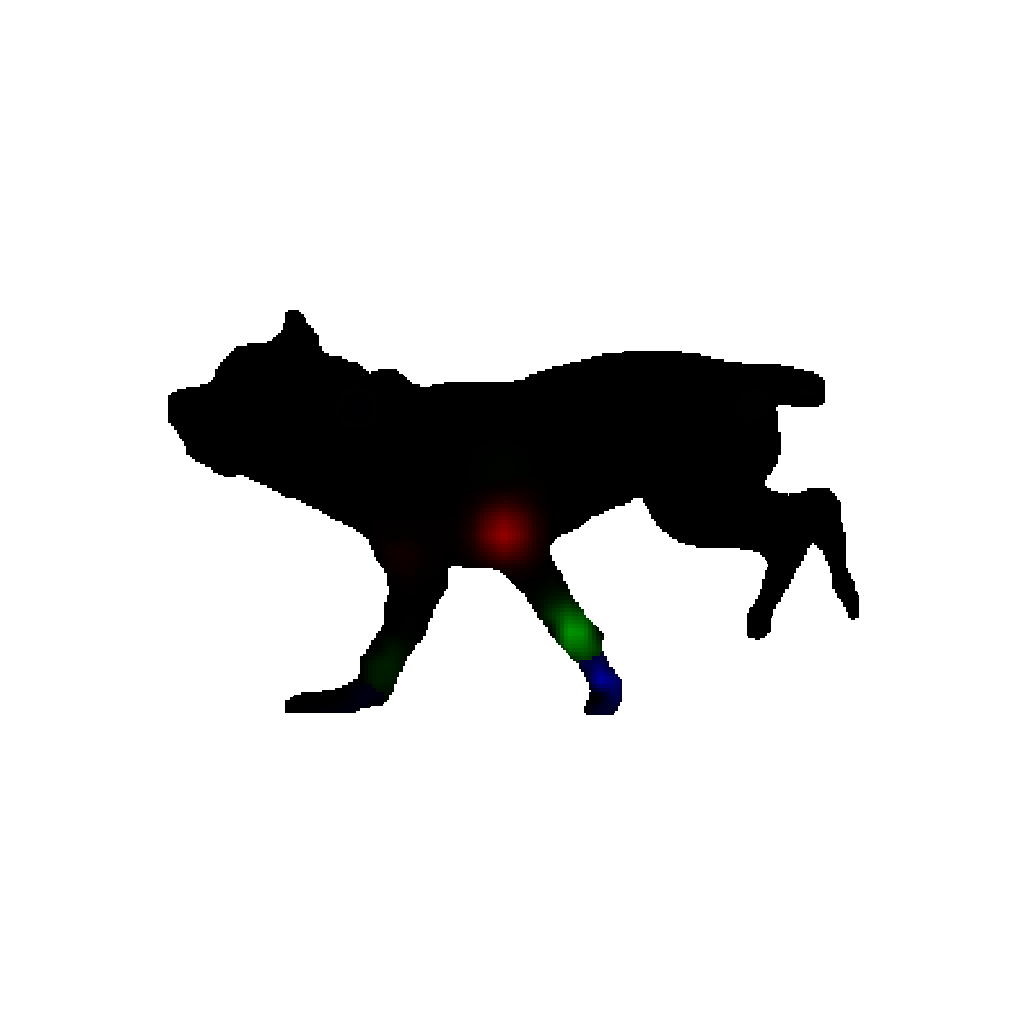
\includegraphics[trim={4cm 10cm 4cm 10cm},clip,width=0.5\linewidth]{single_vs_multi_new/left_heatmap_single.png} &
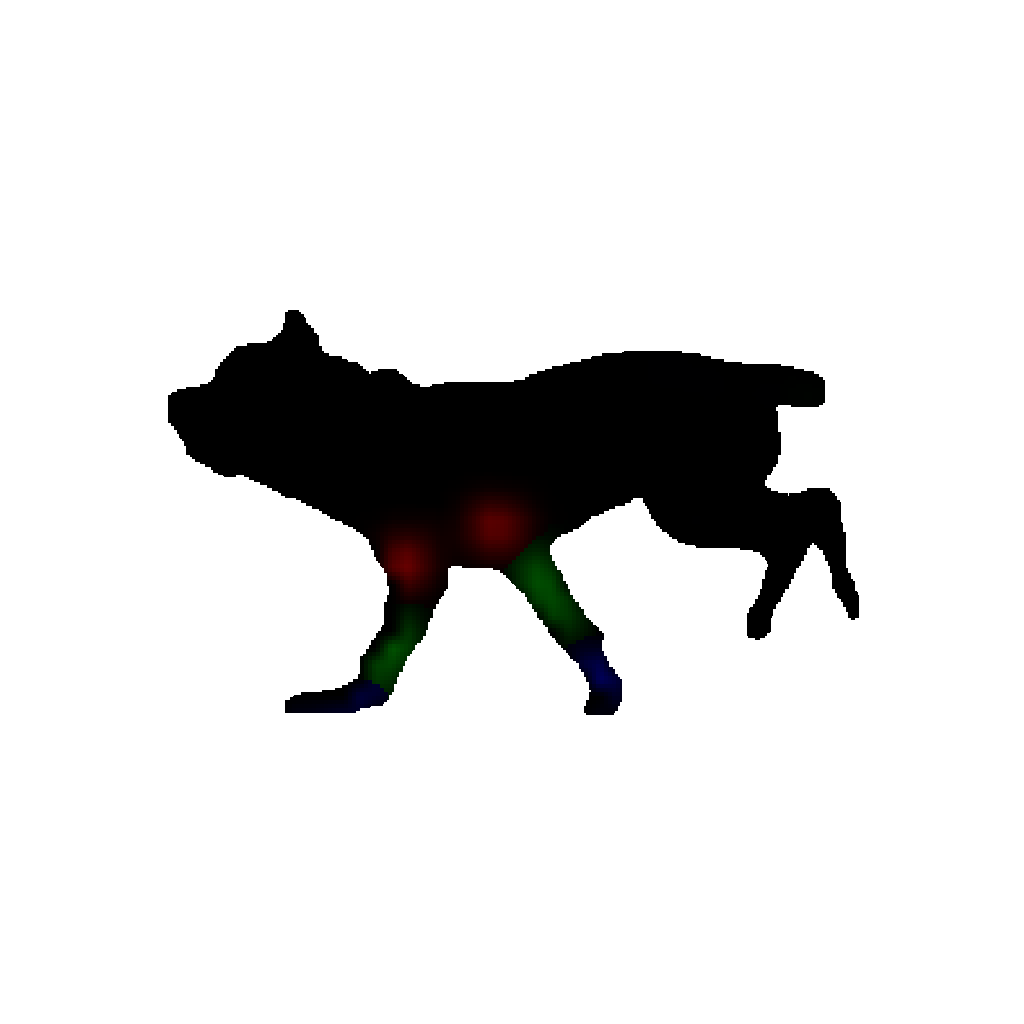
\includegraphics[trim={4cm 10cm 4cm 10cm},clip,width=0.5\linewidth]{single_vs_multi_new/left_heatmap_multi.png} \\
\end{tabular}
% }
{
\caption{Example predictions from a network trained on unimodal (top) and multi-modal (bottom) ground-truth  for front-left leg joints.}
\label{fig:single_multi}
}
% \end{floatrow}
\end{figure}

\begin{figure}[t]
% \begin{floatrow}
% \ffigbox{
\centering
\def\lp#1#2{\labelledpic{\includegraphics[width=0.20\linewidth]{#2}}{#1}}
\begin{tabular}{cccc}
\lp a{skeletons_new/skeleton_rgb_dog_cropped.jpg}&
\lp b{skeletons_new/skeleton_rgb_impala_cropped.jpg}&
\lp c{skeletons_new/skeleton_rgb_rhino_cropped.jpg}&
\lp d{skeletons_new/skeleton_rgb_horsejump-high_cropped.jpg}\\
\end{tabular}
% }
{
\caption{Example outputs from the joint prediction network, with maximum likelihood predictions linked into skeleton.}
\label{fig:exp-network}
}
% \end{floatrow}
\end{figure}

\section{Optimal joint assignment (OJA)}\label{sec:qp}

Since heatmaps generated by the joint predictor are multi-modal, the non-maximum suppression procedure yields multiple possible locations for each joint. The set of joint proposals is represented as $X = \{x_{jp}\}$, where $x_{jp}$ indicates the 2D position of proposal $p \in \{1,...,N_j\}$ associated with joint $j \in J$.
Before applying the optimizer, a subset of proposals $X^* \subseteq X$ should be selected in order to form a complete skeleton, i.e. precisely \emph{one proposal is selected for every joint}. This section will consider how to choose the optimal subset by formulating the problem as an extended optimal assignment problem.

In order to select a complete skeleton proposal from the set of joint proposals $\{x_{jp}\}$, a binary indicator vector $\bvec a_j = \{a_{jp}\} \in \{0, 1\}^{N_j+1}$ is introduced, where $a_{jp} = 1$ indicates that the $p^\text{th}$ proposal for joint $j$ is a correct assignment, and the $p = N_j+1$ position corresponds to a {\em null proposal}, indicating that joint $j$ has no match in this image.
The null proposals are handled as described in each of the energy terms below.
Let $A$ be the jagged array $[\bvec a_j]_{j=1}^J$ containing all assignment variables (for the current frame), and let $X^* = X(A)$ denote the subset of points selected by the binary array $A$.


% Please add the following required packages to your document preamble:
% \usepackage{booktabs}
% \usepackage{multirow}
\begin{table}
    \RawFloats
    \parbox{.48\linewidth}{
        \strut
        \centering
        \begin{tabular}{@{}llll@{}}
        \toprule
        Joint $j$               & Proposal $p$ & $x_{jp}$ & $a_{jp}$ \\ 
        \midrule
        \multirow{3}{*}{Nose} & 0          & $(0, 2) $   & 1 \\
                            & 1          & $(4, 2) $   & 0 \\
                            & NULL       & ---         & 0 \\
        \midrule
        Upper Leg             & NULL       & ---         & 1 \\
        \midrule
        \multirow{3}{*}{Paw}  & 0          & $(4, 2)$    & 0 \\
                            & 1          & $(8, 10)$   & 1 \\
                            & NULL       & ---         & 0 \\
        \midrule
        \multirow{4}{*}{Tail} & 0          & $(4, 2)$    & 0 \\
                            & 1          & $(8, 10)$   & 0 \\
                            & 2          & $(4, 2)$    & 1 \\
                            & NULL       & ---         & 0 \\
        \bottomrule
        \end{tabular}
        \caption{Example inputs and output to the joint assignment problem. Non maximum suppression applied to predicted heatmap tensors yields a set of proposals $p$ for each each skeleton joint $j$ at 2D location $x_{jp}$. $a_{jp}$ is an illustrative assignment vector which is predicted by the OJA algorithm.}
        \label{tab:oja-example-inputs}
    }
    \hfill
    \parbox{.48\linewidth}{
        \strut
        \centering
        \parbox{\linewidth}{
            \strut
            \centering
            \begin{tabular}{@{}lllll@{}}
            \toprule
            Joint $j$ & \multicolumn{4}{l}{Proposal $p$}                                                 \\
            \midrule
            Nose      & 1 & 0                        & 0                        & \cellcolor[HTML]{808080} \\
            Upper Leg & 1 & \cellcolor[HTML]{808080} & \cellcolor[HTML]{808080} & \cellcolor[HTML]{808080} \\
            Paw       & 0 & 1                        & 0                        & \cellcolor[HTML]{808080} \\
            Tail      & 0 & 0                        & 1                        & 0                        \\
            \bottomrule
            \end{tabular}
            \caption{Assignment variables $A = \bvec a_j = \{a_{jp}\} \in \{0, 1\}^{N_j+1}$ for the current frame stored as a jagged array.}
            \label{tab:oja-proposals}
        }
        \bigskip
        \parbox{\linewidth}{
            \strut
            \centering
            \begin{tabular}{@{}ll@{}}
                \toprule
                Joint $j$ & $X^* = X(A)$ \\
                \midrule
                Nose      & $(0, 2)$     \\
                Upper Leg & ---          \\
                Paw       & $(8, 10)$    \\
                Tail      & $(4, 2)$     \\
                \bottomrule
            \end{tabular}
            \caption{2D joint locations $X^* = X(A)$ selected by the assignment variable $A$}
            \label{tab:oja-selected}
        }
    }
\end{table}        
        

Optimal assignment minimizes the function
\begin{equation}
L(A) = \LL{conf}(A) + \LL{null}(A) + \LL{prior}(A) + \LL{temp}(A) + \LL{cov-sil}(A) + \LL{cov-bone}(A)
\end{equation}
which balances agreement of the joint configuration with the network-supplied {\em confidences}, a learned {\em prior}, {\em temporal} coherence, and {\em coverage} terms which encourage the model to correctly project over the silhouette. Without the coverage terms, this can be optimized as a quadratic program, but better results are obtained by including the coverage terms, and using a genetic algorithm. In addition, the parameters $A$ must satisfy the $J$ constraints $\sum_{p=1}^{N_j+1} a_{jp} = 1$, that exactly one joint proposal (or the null proposal) must be selected for each joint.

\subsection{Basic formulation}

\subsubsection{Network confidences: $\LL{conf}(A)$}

The first energy term $\LL{conf}(A)$ comes from the output of the joint prediction network, which provides a confidence score $y_{jp}$ associated with each joint proposal~$x_{jp}$.  Then $\LL{conf}(A) = \sum_j\sum_p -\lambda_{\text{conf}}\log(y_{jp}) A_{jp}$ is a linear function of $A$, 
and $\lambda_{\text{conf}}$ is a tunable parameter to control the relative contribution of the network confidences compared with that of the skeleton prior. Note that if only this term is included, the OJA would simply produce the result of the standard non-maximal suppresion algorithm, selecting the heatmap location with highest network confidence. Note that this function can be rewritten as

\begin{equation}\label{eq:conf-energy}
    \LL{conf}(A) = \lambda_{\text{conf}}\log(y^T) \text{vec}(A)
\end{equation}

\subsubsection{Null proposals: $\LL{null}(A)$}

Under some circumstances, for example when a body part is heavily occluded or ambiguous, \emph{all} available proposals for a given joint may be of poor quality. In such a case, including any of these options in a skeleton configuration may have a detrimental impact on the later model fitting stage. Under these circumstances, it may be preferable to exclude the joint in question from the optimization entirely. Null proposals pay a fixed cost $\lambda_{null}$, effectively acting as a threshold whereby the null proposal will be selected if no other proposal is of sufficient likelihood. Precisely, a jagged array $D$ is defined

\begin{equation}
    D_{jp} = \begin{cases}
        \lambda_{\text{null}} & \text{if } p \text{ is null proposal}\\
        0 & \text{otherwise}
    \end{cases}
\end{equation}

and resulting energy becomes

\begin{equation}\label{eq:null-energy}
    \LL{null}(A) = \text{vec}(D) \text{vec}(A)
\end{equation}

\subsubsection{Skeleton Prior: $\LL{prior}(A)$}

The next energy term is used to discourage anatomically implausible skeletal configurations from being selected. The prior probability of a skeletal assignment $A$ is represented as a multivariate Gaussian distribution over the selected joint positions $X^* = X(A)$

% % Here, x is used as a general 2D coordinate
\begin{equation}
P_{\mathrm{prior}}(A) = \frac{1}{\sqrt[]{(2\pi)^k\left|\Sigma\right|}}\exp\left(-\frac{1}{2}(x^*-\mu)^T\Sigma^{-1}(x^*-\mu)\right)
\end{equation}

The mean $\mu \in \R{2J}$ and covariance $\Sigma \in \R{2J\times 2J}$ terms are obtained from synthetic training examples generated earlier. The prior is shown in \Cref{fig:skeleton-prior}. The objective of the OJA is to find the assignment vector $A$ which maximizes this prior, which is equivalent to minimizing the negative log prior
\begin{equation}
    \LL{prior}(A) = \frac{k}{2}\log(2\pi) + \frac{1}{2}\left|\Sigma\right| + \frac{1}{2}(x^*-\mu)^T\Sigma^{-1}(x^*-\mu)
\end{equation}

This formulation is reducible to a minimization over the Mahalanobis distance, which is given by the summation
\begin{equation}
\LL{prior}(A) = \sum_j^J\sum_p^{N_j}\sum_k^J\sum_q^{N_k}a_{jp}a_{kq}(x_{jp} - \mu_j)\Sigma_{jk}^{-1}(x_{kq}-\mu_k)
\end{equation}

Notice this is a quadratic function of $A$, so $\LL{prior}(A) = \text{vec}(A)^\top Q \text{vec}(A)$ for a fixed matrix $Q$. Precisely, the elements of the matrix $Q$ are precisely the Mahalanobis distance between each individual pair of joint proposals
\begin{equation}
\left[Q\right]_{jp, kq} = (x_{jp} - \mu_j)\Sigma_{jk}^{-1}(x_{kq}-\mu_k)
\end{equation}

Null proposals are simply excluded from the sum, equivalent to marginalizing over their position. 


\begin{figure}[t]
\def\bb{\rule{2in}{0pt}\rule{0pt}{1in}}
\begin{tabular}{cccc}
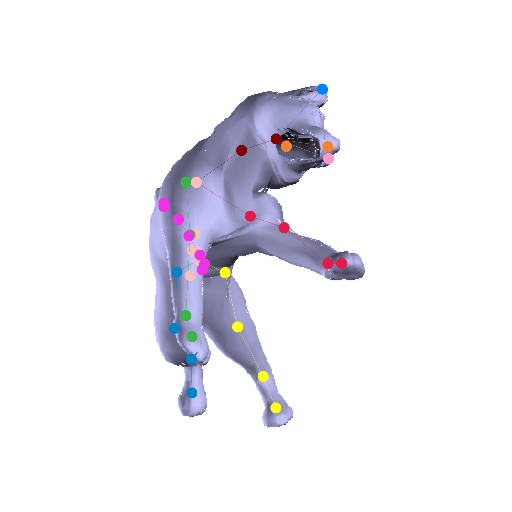
\includegraphics[width=0.25\linewidth]{skeletal_prior_gen/63_rgb.png} & 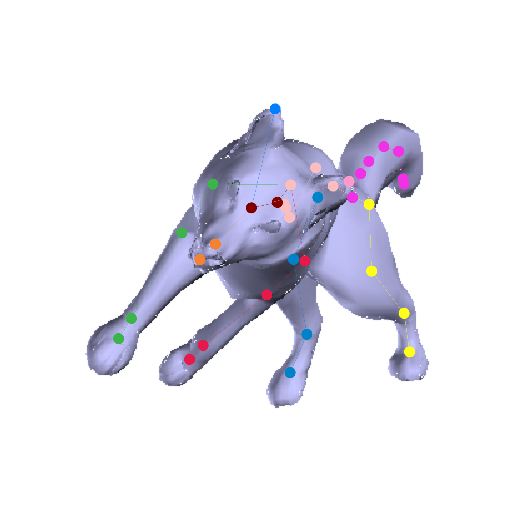
\includegraphics[width=0.25\linewidth]{skeletal_prior_gen/36_rgb.png} & 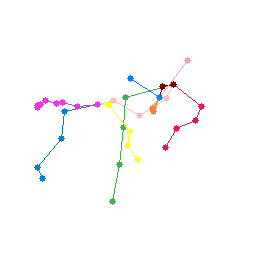
\includegraphics[width=0.25\linewidth]{skeletal_prior/74.png} & 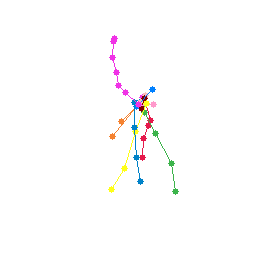
\includegraphics[width=0.25\linewidth]{skeletal_prior/108.png} \\
(a) & (b) & (c) & (d) \\
\end{tabular}
\caption{Skeleton Prior: Synthetic quadruped training data examples (rendered with texture to show 3D) generated by sampling pose, shape and position parameters and applying to SMAL model (a), (b). The set of 2D skeletal positions are used to create a vector of means $\mu \in \mathbb{R}^{2J}$ and covariance matrix $\Sigma \in \mathbb{R}^{2J \times 2J}$. The Gaussian distribution constructed can be sampled to create new skeletons, such as those shown in (c), (d).}
\label{fig:skeleton-prior}
\end{figure} 

\subsubsection{Temporal Prior: $\LL{temp}(A)$}
% TODO: Consider bringing in qp_defs/IMAGES to help explain and draw matrices Q
A common failure case of the joint prediction network is in situations where a joint position is highly ambiguous, for example between the left and right legs. In such cases, the algorithm will commonly alternate between two equally likely predictions. This leads to large displacements in joint positions between consecutive frames which are difficult for the later model fitting stage to recover from. This can be addressed by introducing a temporal term into the OJA. A prior is imposed on the distance moved by each joint between frame $t_0$ and $t_1$, which is given by a normal distribution with zero mean and variance $\sigma^{2} =e^{\tau|t_1 - t_0 - 1|}$. 
The parameter $\tau$ controls the strength of the interaction between distant frames. This results in an additional quadratic term in our objective function, which has the form $L_{temp} = a^\top T^{(t_0, t_1)} a$ for matrix $T^{(t_0, t_1)}$ given by 
\begin{equation}
\left[T^{(t_0, t_1)}\right]_{jp, kq} = \begin{cases}
e^{-\alpha|t_1 - t_0 - 1|}||x^{(t_0)}_{jp} - x^{(t_1)}_{kq}||^2 & \text{if } j=k\\
0 & \text{otherwise}
\end{cases}
\end{equation}

\subsection{QP solution.}
A general quadratic program is made up of a quadratic objective function and linear equality and inequality constraints. Thus far, all terms in $L(A)$ are quadratic or linear. 

To optimize over a sequence of frames, we construct the block diagonal matrix $\hat{Q}$ whose diagonal elements are the prior matrices $Q^{(t)}$ and off-diagonal elements are the temporal matrices $T^{(t_0, t_1)}$. The confidence term \Cref{eq:conf-energy} and null penalty term \Cref{eq:null-energy} are combined and the vector $\hat{c}$ is obtained by stacking across each frame. The solution vector for the sequence $\hat{a}$ is similarly constructed by stacking the vectorized assignment matrices $A$ across timesteps. The jagged array $B$ is used to formalize the constraint that only one proposal should be selected per joint. Precisely

\begin{equation}
    \left[B\right]_{jp,kq} = \begin{cases}
        1 & \text{if } j=k\\
        0 & \text{otherwise}
    \end{cases}
\end{equation}
and (similarly to $A$) is vectorized and stacked across timesteps to form the constraint $\hat{B}\hat{a} = 1$. Finally, the constraint $\hat{a}(1 - \hat{a})=0$ is applied to ensure binary values of $\hat{a}$. The resulting quadratic program formulation is then given in \Cref{eq:quadprog}.



% \begin{equation}
% \min_{\hat{a}} \quad \hat{a}^T \hat{Q} \hat{a} + \lambda_{temp} \hat{a}^T \hat{T} \hat{a} + \lambda_{conf} \hat{c}_{conf}^T \hat{a} + \lambda_{null} \hat{c}_{null}^T\hat{a}
% \end{equation}

% \[
% \begin{array}{c c} &
%     \begin{array}{c c c} p=1 & p=2 & p=3 \\
%     \end{array}
%     \\
%     \begin{array}{c c c}
%     p=1 \\
%     p=2\\
%     p=3
%     \end{array}
%     &
%     \left[
%     \begin{array}{c c c}
%     0.1 & 0.1 & 0.0 \\
%     0.4 & 1.0 & 0.0 \\
%     0.8 & 0.0 & 0.4
%     \end{array}
%     \right]
% \end{array}
% \]

\begin{mini}
    {\hat{a}}{\hat{a}^T \hat{Q} \hat{a} + \hat{c}^T \hat{a}}{}{}
    \addConstraint{\hat{B}\hat{a} = 1}
    \addConstraint{\hat{a}(1 - \hat{a}) = 0}
    \label{eq:quadprog}
\end{mini}

% \begin{align}
%     \min_{\hat{a}} \quad \hat{a}^T \hat{Q} \hat{a} + \lambda_{temp} \hat{a}^T \hat{T} \hat{a} + \lambda_{conf} \hat{c}_{conf}^T \hat{a} + \lambda_{null} \hat{c}_{null}^T\hat{a} \\
%     \text{subject to } \sum_p^{N_j} \hat{a}_{jp} = 1 \quad \forall j & \quad \text{and } \hat{a}_{jp}(1 - \hat{a}_{jp}) = 0 \quad \forall j,p 
    
% \end{align}

The quadratic program is specified using the open source CVXPY library \cite{diamond2016cvxpy} and solved using the ``\emph{Suggest-and-Improve}'' framework proposed by Park and Boyd \cite{park2017general}. It is initialized by choosing the proposal with the highest confidence for each joint. Appropriate values for the free parameters $\lambda_{\text{conf}, \text{temp}, \text{null}}$ and $\alpha$ were chosen empirically via grid search. 

\subsection{Incoporating coverage priors}

The above quadratic formulation is sufficient to correct many errors in the raw output (which we later demonstrate in the experimental section), but suffers from an `overcounting' problem, in which leg joint predictions both cover the same silhouette leg region, leaving another leg empty. We therefore extend the definition of $L(A)$ to include two additional terms. 

\def\silhouette{S}

\subsubsection{Silhouette coverage: $\LL{cov-sil}$}

The silhouette coverage term is designed to penalize large silhouette areas with no nearby selected joint. This term requires a precomputed set of silhouette sample points $Z \subseteq \mathbb{R}^2$, which we aim to ``cover'' as best as possible with the set of selected joints. Intuitively, the silhouette is considered well-covered if all sample points are close to \emph{some} selected joint proposal. The set $Z$ is generated from the medial axis transform (MAT)\cite{blum1967transformation} of the silhouette, $Z^{t} = \text{MAT}(\silhouette^{t})$
with a cubed loss strongly penalizing projection outside the silhouette:
\begin{equation}
\LL{cov-sil}(A^{t};X^{t},Z^{t}) = \sum_{i}\min_{j}\|Z_{i}^{t} - \hat{X}_{j}^{t}\|^3
\end{equation}

\begin{figure}[t!]
\begin{floatrow}
\ffigbox{%%%%%%%%%%%%
\def\bb{\rule{2in}{0pt}\rule{0pt}{1in}}
\def\bjb{\rule{0.5in}{0pt}\rule{0pt}{0.25in}}

\begin{center}
\scalebox{-1}[1]{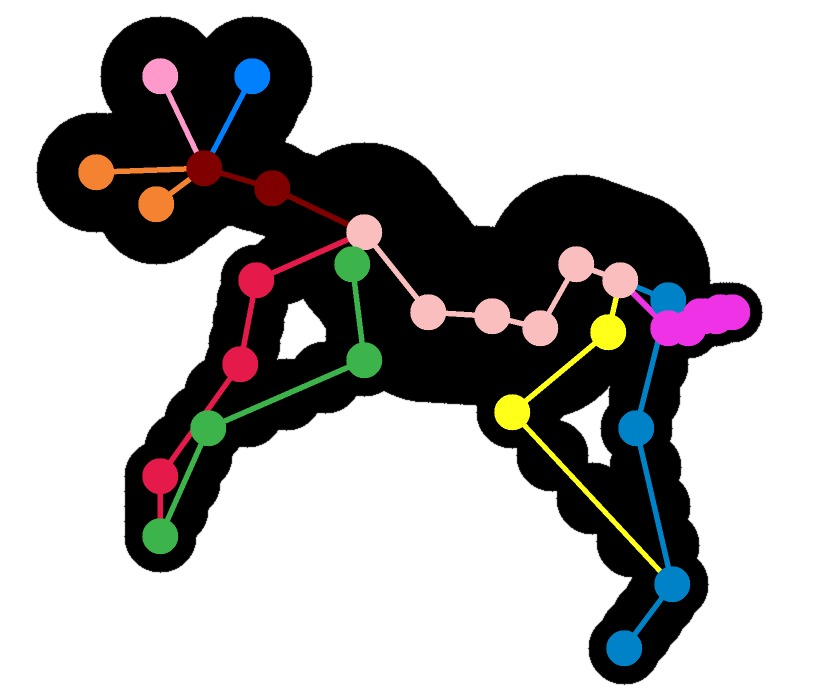
\includegraphics[width=0.49\linewidth]{sil_coverage_new/approx_render_cov_cropped.jpg}}
\scalebox{-1}[1]{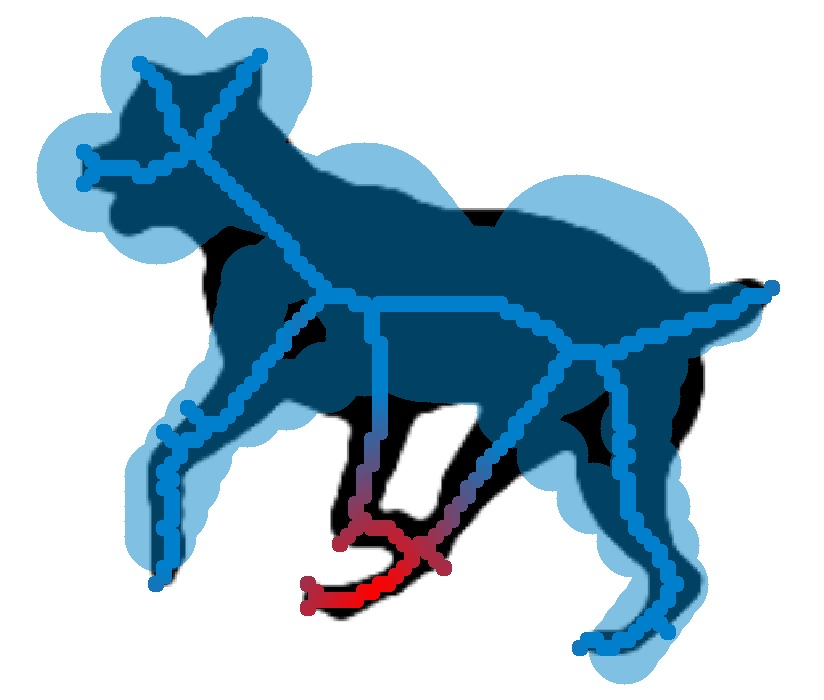
\includegraphics[width=0.49\linewidth]{sil_coverage_new/med_axis_overlay_error_cropped.jpg}}
% predictions taken from rs_dog frame 0100
\end{center}
}
{\caption{Silhouette coverage loss. The error (shown in red) is the the distance between the median axis transform (right) and the nearest point on an approximate rendering (left).}
\label{fig:example_errors}}
\ffigbox{ 
    \raisebox{1 em}{
    \centering
    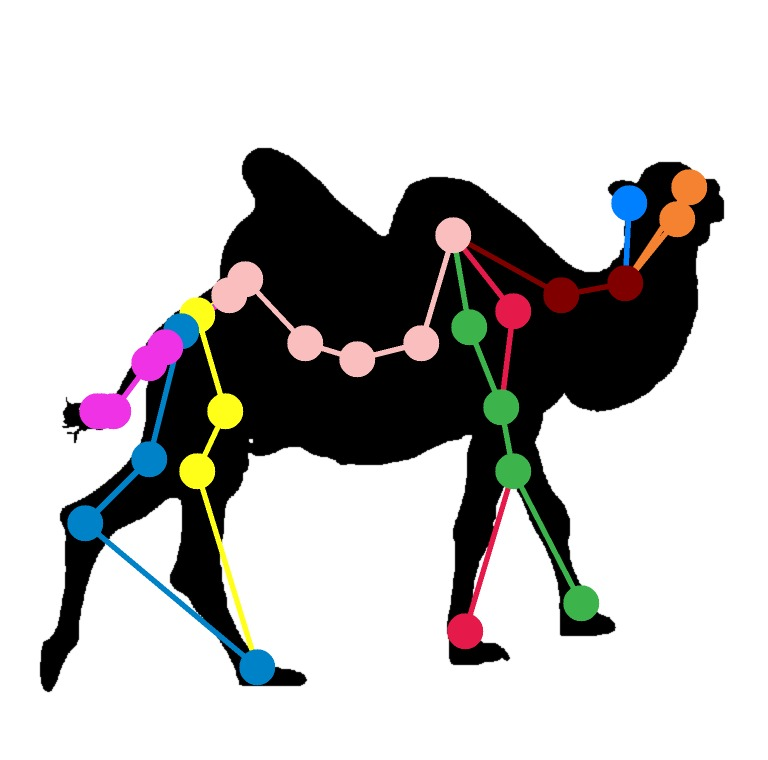
\includegraphics[trim={0cm 0cm 0cm 0cm}, clip,width=0.45\linewidth]{bone_coverage/skeleton_sil_cropped.jpg}
    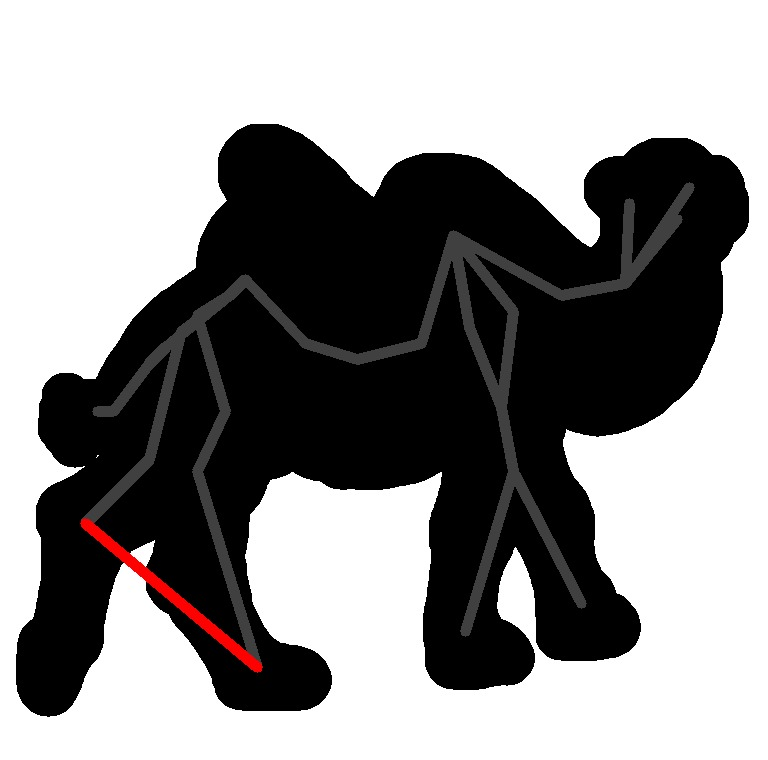
\includegraphics[trim={0cm 0cm 0cm 0cm},clip,width=0.45\linewidth]{bone_coverage/bone_error_overlay_cropped.jpg}
    }
}
{\caption{Bone coverage loss. One of the back-right leg joints is incorrectly assigned (left), leading to a large penalty since the lower leg bone crosses outside the dilated silhouette (right).}
\label{fig:cov-bone}
% camel 0020}
}
\end{floatrow}
\end{figure}

\subsubsection{Bone coverage: $\LL{cov-bone}$}

The bone coverage term is used to prevent bones crossing the background. The joint hierarchy is stored in a kinematic tree structure $K = \{\{j,k\} \text{ if joints } j, k \text{ are connected by a bone}\}$.
\begin{equation}
\LL{cov-bone}(A^{t};X^{t},\silhouette^{t},K) = \sum_{\{j,k\} \in K}\biggl(1 - \min_{\lambda \in \big[0:0.1:1\big]}\silhouette^{t}(\hat{X}_{j}^{t} + \lambda(\hat{X}_{j}^{t} - \hat{X}_{k}^{t}))\biggr)
\end{equation}

\subsection{Formulation as a genetic algorithm}
We minimize this more complex objective using a genetic algorithm (GA)\cite{holland1992adaptation}. A genetic algorithm is a method for solving optimization problems using a natural selection process that mimics biological evolution. Unlike the quadratic program described previously, the GA optimization procedure relies on crossover and mutation, rather than by calculating derivatives. In some cases (and as shown in this work), this can lead to much faster convergence properties. The following components are required:

\ss{Genes.} Candidate solutions to the optimization problem are referred to as a set of `genes'. In this case, a gene is the asssignment array $A$ although is represented as a vector of $J$ integers (indicating the proposal ID), rather than one-hot encodings. 

\ss{Initial population.} Genes are constructed subject to the constraints given in \Cref{eq:quadprog}. The genetic algorithm is initialized with a population size of 128 genes. Of these, the first 32 are set equal to the max confidence solutions given by the network, which speeds up convergence. The remaining 96 genes are generated by selecting a random proposal for each joint. 

\ss{Fitness function.} A fitness function is used to evaluate the quality of a gene. In this setting, the fitness function is precisely the energy $L(A)$ given above which minimizes to yield an optimal skeleton configuration.

\ss{Crossover.} Crossover is a fundemental operation common to evolutionary methods which defines the process of combining the information of two `parent' genes to generate an offspring gene. \emph{Single-point} crossover operates by slicing parent genes each into two parts, and combining first and second parts from different parents to yield the next generation. Following standard practice, the crossover point is randomly selected for each combination. 

\ss{Mutation.} Analogous to biological mutation and used to maintain diversity among genes, each gene is assigned some probability of undergoing a {\em mutation}. If a gene 
is selected for mutation, between 1 and 4 joints have new proposals randomly assigned.

The genetic algorithm described has weights set empirically and is run for 1000 generations. Examples of errors corrected by the additional coverage energy terms are shown in Fig.~\ref{fig:example_errors} and Fig.~\ref{fig:cov-bone}.


\section{3D model fitting}
The model optimization stage refines model parameters to match the silhouette sequence $\mathcal S$. The procedure defined here is inspired by the human reconstruction method of SMALify~\cite{bogo16keep} (defined in detail in \Cref{chap:relwork}) and the non-automatic quadruped fitting method presented in 3D Menagerie (3DM) ~\cite{zuffi2017menagerie}. The technique presented in this section can be viewed as an extension of these approaches to input video sequences. 

% SMALR exploited this fact (simultaneous fitting) in tangential work to ours.
A naive 3D model fitting implementation would be to simple apply 3DM independently to each of the $N$ video frame to yield a set of pose parameters $\seq{\pose}{t}{1}{N}$, shape parameters $\seq{\shape}{t}{1}{N}$ and position parameters $\seq{\posn}{t}{1}{N}$. However, fitting to a video sequence rather than single frames offers additional opportunities to constrain the challenging monocular 3D reconstruction task. For example, video sequences typically offer multiple views of the animal subject, although the animal's limb positions often change between frames. However, the animal's \emph{shape} characteristics (such as height, body proportions etc.) can be relied upon to remain largely consistent between frames. This fact is exploited through an extension that learns a single set of \emph{global} shape parameters $\shape$ and is assigned to across all frames $\shape_{t} := \shape$. Another benefit offered by video is the opportunity to constrain inter-frame subject motion. Assuming a reasonable framerate, it is expected that the animal's pose and position parameters should vary only slightly between successive frames. This intuition is characterized in \Cref{eq:temporal-energy}.

The following section defines the 4 energy terms used in the optimization: 

\ss{Silhouette energy.}
The silhouette energy $\E{sil}$ compares the 3D animal model to the silhouette image according to the L2 distance between the OpenDR rendered binary image and the input silhouette:

\begin{equation}
\E{sil}(\posn_{t}, \pose_{t}, \shape; S_{t}) = \lVert S_{t} - R\bigl(\posn_{t} * \verts(\pose_{t}, \shape)\bigr) \rVert
\end{equation}

\ss{Unimodal Prior energy.}
The prior term $\E{prior}$ encourages the regressed shape and pose parameters to remain close to a those in the combined artist traininthose in our set of artist 3D dog meshes.

% \begin{equation}
%     \L{pose}(\pose) = (\pose - \meanpose)^T \pose_cov^{-1} (\pose - \meanpose)
% \end{equation}

% \begin{equation}
%     \L{uni-shape}(\beta) = (\beta - \meanbeta)^T \beta_cov^{-1} (\beta - \meanbeta)
% \end{equation}

The Mahalanobis distance is used to encourage the model to remain close to: (1) a distribution over shape coefficients given by the mean and covariance of SMAL training samples of the relevant animal family, (2) a distribution of pose parameters built over a walking sequence. The final term ensures the pose parameters remain within set limits.
\begin{equation}
\E{lim}(\pose_{t}) = \max\{\pose_{t} - \pose_{\text{max}}, 0\} + \max\{\pose_{\text{min}} - \pose_{t}, 0\}.
\end{equation}

\ss{Joints energy.}
The joints energy $\E{joints}$ compares the rendered model joints to the OJA predictions, and therefore must account for missing and incorrect joints.  It is used primarily to stabilize the nonlinear optimization in the initial iterations, and its importance is scaled down as the silhouette term begins to enter its convergence basin.

\begin{equation}
\E{joints}(\posn_{t}, \pose_{t}, \shape; X^{*}) = 
\lVert X^{*} - \posn_{t} * \verts(\pose_{t},\shape)\jointselect_{t}(:,j) \rVert
\end{equation}

\ss{Temporal energy.}
The optimizer for each frame is initialized to the result of that previous. In addition, a simple temporal smoothness term is introduced to penalize large inter-frame variation:
\begin{equation}
\E{temp}(\posn_{t}, \pose_{t}) = (\posn_{t} - \posn_{t+1})^2 + (\pose_{t} - \pose_{t+1})^2
\end{equation}\label{eq:temporal-energy}

% TODO: Maybe some more here?
The optimization is via a second order dogleg method~\cite{lourakis2005levenberg}.


\section{Experiments}
This section details both quantitative and qualitative evaluation of the system described in the previous sections. Due to the lack of animal keypoint datasets in the public domain, it is necessary to construct a new Benchmark Animal Dataset of Joint Annotations (BADJA). BADJA is a dataset comprising several video sequences with hand-clicked 2D joint labels and segmentation masks. Qualitative results are provided on BADJA and also on images used in the evaluation of 3D Menagerie (3DM). However, it should be noted this comparison is not entirely fair, since 3DM requires hand-clicked keypoints as input and system introduced in this chapter is optimized for video input.

\subsection{BADJA Dataset}
The BADJA dataset contains 9 videos, with manually collected keypoint and silhouette annotations. 7 video sequences were obtained from the DAVIS video segmentation dataset~\cite{Perazzi2016} and came with existing silhouettes, and the remainder were sourced from online stock footage. Segementation masks for these were generated using Adobe's UltraKey tool~\cite{adobe_ultrakey}. For all sequences, a set of 20 joints were labelled as illustrated in \figref{badja_examples}. The first 16 joints are located on legs, neck and tail, and defined by the rigged 3D SMAL skeleton. The final joints (nose tip, chin and ears) do not directly relate to 3D SMAL joints, but are instead defined by particular SMAL model vertices. A similar trick is used in SMALify~\cite{bogo16keep} to indicate the position of the human nose which has no corresponding SMPL joint. The collection of joints were chosen on the basis of being of informative to the skeleton and being simple for a non-expert human annotator to localize. To make manual annotation feasible and to ensure a diverse set of data, annotations are provided for every fifth video frame and were collected using the excellent LabelMe tool~\lazycite{LabelMe}{LabelMe}. 

The video sequences were selected to comprise a range of different quadrupeds undergoing various movement typical of their species. Although the dataset is perhaps insufficient in size to train deep neural networks, the variety in animal shape and pose renders it suitable for evaluating quadruped joint prediction methods. 

\subsection{Joint prediction}
\label{sec:exp-network}
%bjb_insert
For the joint predictor $\rho$ the stacked hourglass network~\cite{newell2016stacked} modified for multi-modal output is trained on synthetic animal silhouette data. Following state-of-the-art performance on related human 2D pose estimation datasets (\cite{andriluka14cvpr,lin2014microsoft}), the network consists of 8 stacks, 256 features and 1 block. Synthetic silhouette images of size $256\times 256$ are provided as input, which are obtained by randomly sampling shape and pose parameters from the SMAL model. The corresponding training targets are ground truth heatmaps produced by smoothing the 2D projected joint locations with a Gaussian kernel. As a benefit of working with synthetic data, training samples can be generated on the fly, which effectively results in a training set of infinite size. A small adaptation was required to prevent the network degenerating to an unfavourable solution on silhouette input: foreground masks were applied to both ground truth silhouette and predicted heatmaps to prevent the network degenerating to an all-zero heatmap, which produces a reasonably good loss and prevents the network training successfully. The network was trained using the RMSProp optimizer for 40k iterations with a batch size of 18 and learning rate of $2.5\times 10^{-4}$. The learning rate was decayed by 5\% every 10k iterations. Training until convergence took 24 hours on a Nvidia Titan X GPU.

Joint accuracy is evaluated with the Probability of Correct Keypoint (PCK) metric defined by Yang and Ramanan~\cite{yang2013articulated}. The PCK is the percentage of predicted keypoints which are within a threshold distance $d$ from the ground truth keypoint location. The threshold distance is given by $d=\alpha\sqrt{|S|}$ where $|S|$ is the area of the silhouette and $\alpha$ is a constant factor which we set to $\alpha=0.2$ for these experiments.

\figref{exp-network} shows a selection of maximum likelihood joint predictions on real world images. Note that despite being trained only on synthetic data, the network generalizes extremely well to animals in the wild. The performance extends even to species which were not present in the SMAL model, such as the impala and rhino. The network is also robust to challenging poses (\ref{fig:exp-network}b), occlusions (\ref{fig:exp-network}c) and distraction objects such as the human rider in (\ref{fig:exp-network}d). It is however susceptible to situations where the silhouette image is ambiguous, for example if the animal is facing directly towards or away from the camera. Figure~\ref{fig:blooper} contains examples of failure modes.

\begin{figure}[t]
\def\bb{\rule{2in}{0pt}\rule{0pt}{1in}}
\begin{center}
\resizebox{.95\linewidth}{!}{
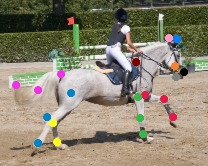
\includegraphics[width=.24\linewidth]{annotations/00110_rgb_horse_cropped.jpg}
~
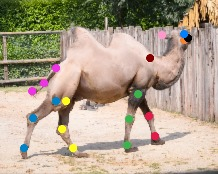
\includegraphics[width=.24\linewidth]{annotations/00021_camel_rgb_cropped.jpg}
~
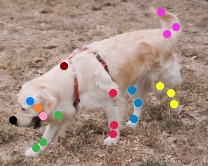
\includegraphics[width=.24\linewidth]{annotations/00085_rgb_dog_cropped.jpg}
~
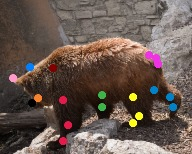
\includegraphics[width=.24\linewidth]{annotations/00008_bear_rgb_cropped.jpg}}
\end{center}
\caption{Example joint annotations from the BADJA dataset.  A total of 11 video sequences are in the dataset, annotated every 5 frames with 20 joint positions and visibility indicators.
}
\label{fig:badja_examples}
\end{figure}

    

\subsection{Optimal joint assignment}
Following non-maximum suppression of the joint heatmaps obtained in Section~\ref{sec:exp-network}, OJA is applied to select an optimal set of joints which initialize the final 3D model fitting stage. It can be seen that the OJA step is able to address many of the failure cases introduced by the joint prediction network, for example by eliminating physically implausible joint configurations (\figref{comparison}, row 1) or by resolving the ambiguity between the left and right legs (\figref{comparison}, row 2).  Table~\ref{tab:animal} summarizes the performance of both the raw network predictions and results of the two OJA methods. Over most of the sequences in the BADJA dataset it can be seen that the use of coverage terms (employed by the OJA-GA model) improves skeleton accuracy. In particular, the bear, camel and rs\_dog sequences show substantial improvements. The method does however struggle on the horsejump\_high sequence, in which part of the silhouette is occluded by the human rider which adversely affects the silhouette coverage term. Across all sequences the selected OJA-GA method improves joint prediction accuracy by 7\% compared to the raw network output. 

\begin{figure}[t]
\begin{floatrow}
\ffigbox{
\def\bb{\rule{2in}{0pt}\rule{0pt}{1in}}
\def\comparisonheight{20mm}
\begin{tabular}{ccc}
    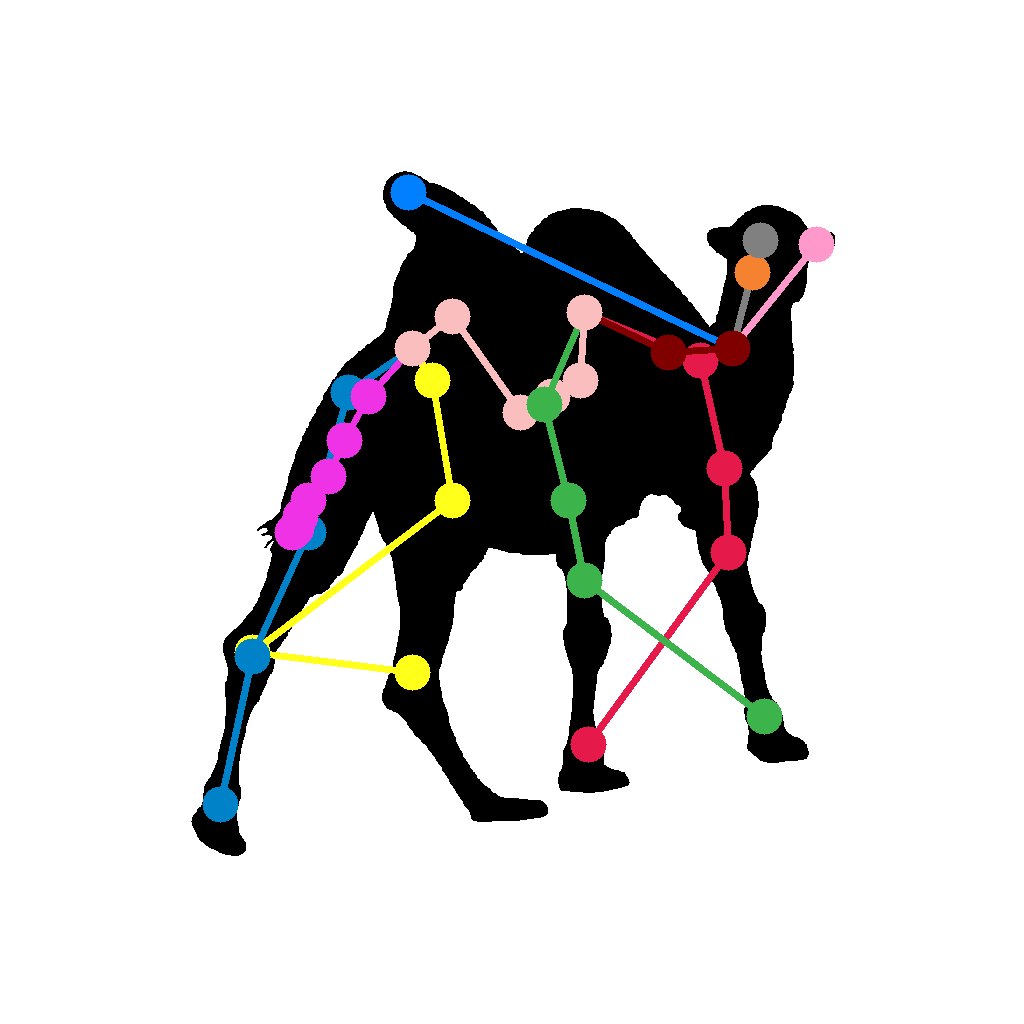
\includegraphics[trim={7cm 6cm 7cm 6cm},clip,height=\comparisonheight]{ga_vs_qp/0046_skel_sil_raw_2.png} &
    
    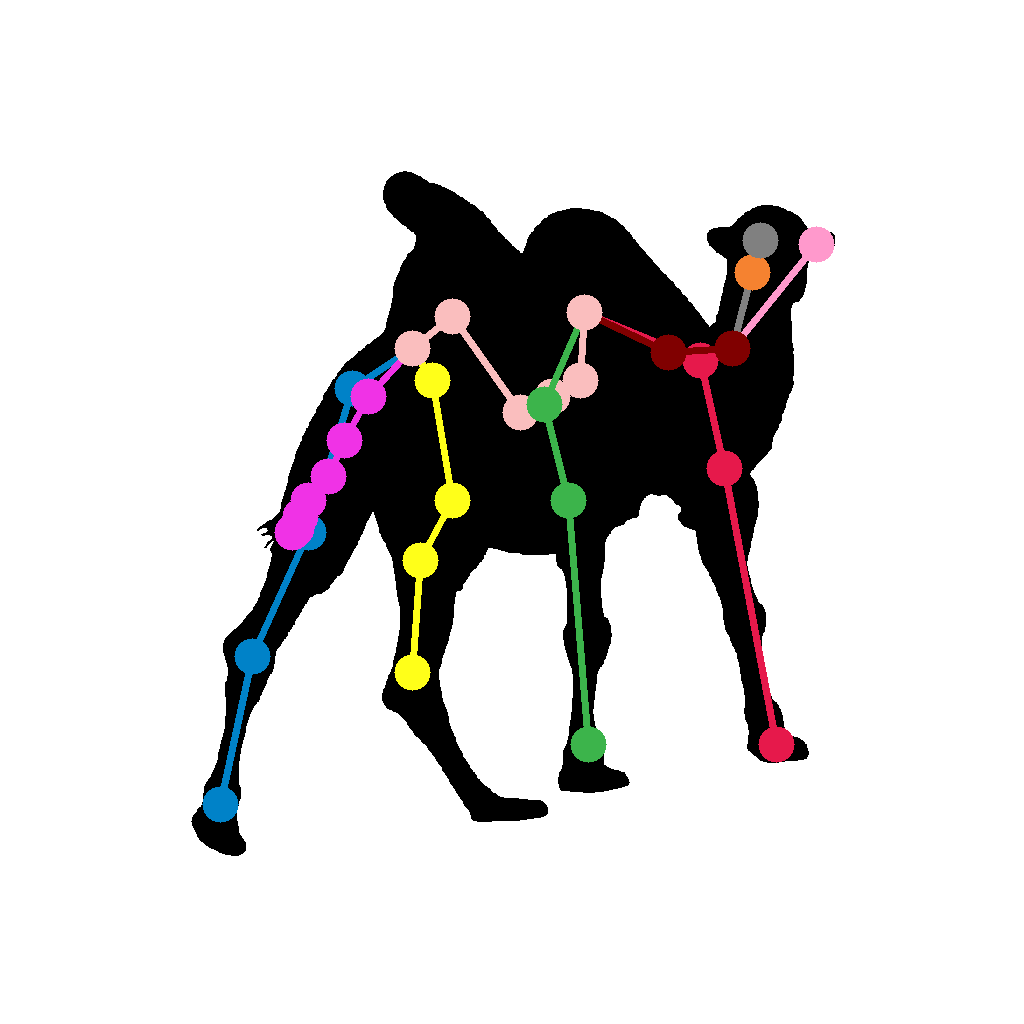
\includegraphics[trim={7cm 6cm 7cm 6cm},clip,height=\comparisonheight]{ga_vs_qp/0046_skel_sil_cleaned_qp_3.png} &
    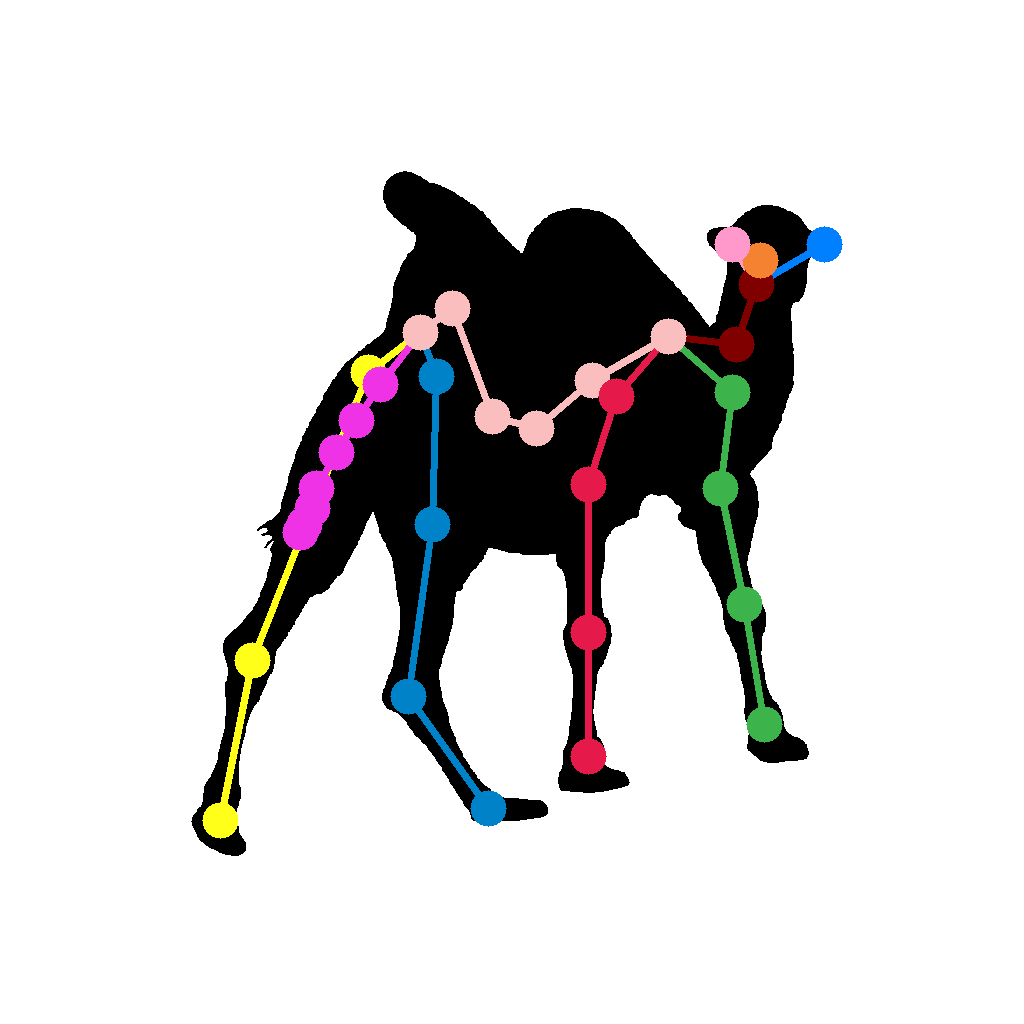
\includegraphics[trim={7cm 6cm 7cm 6cm},clip,height=\comparisonheight]{ga_vs_qp/0046_skel_sil_cleaned_ga_2.png} \\
    
    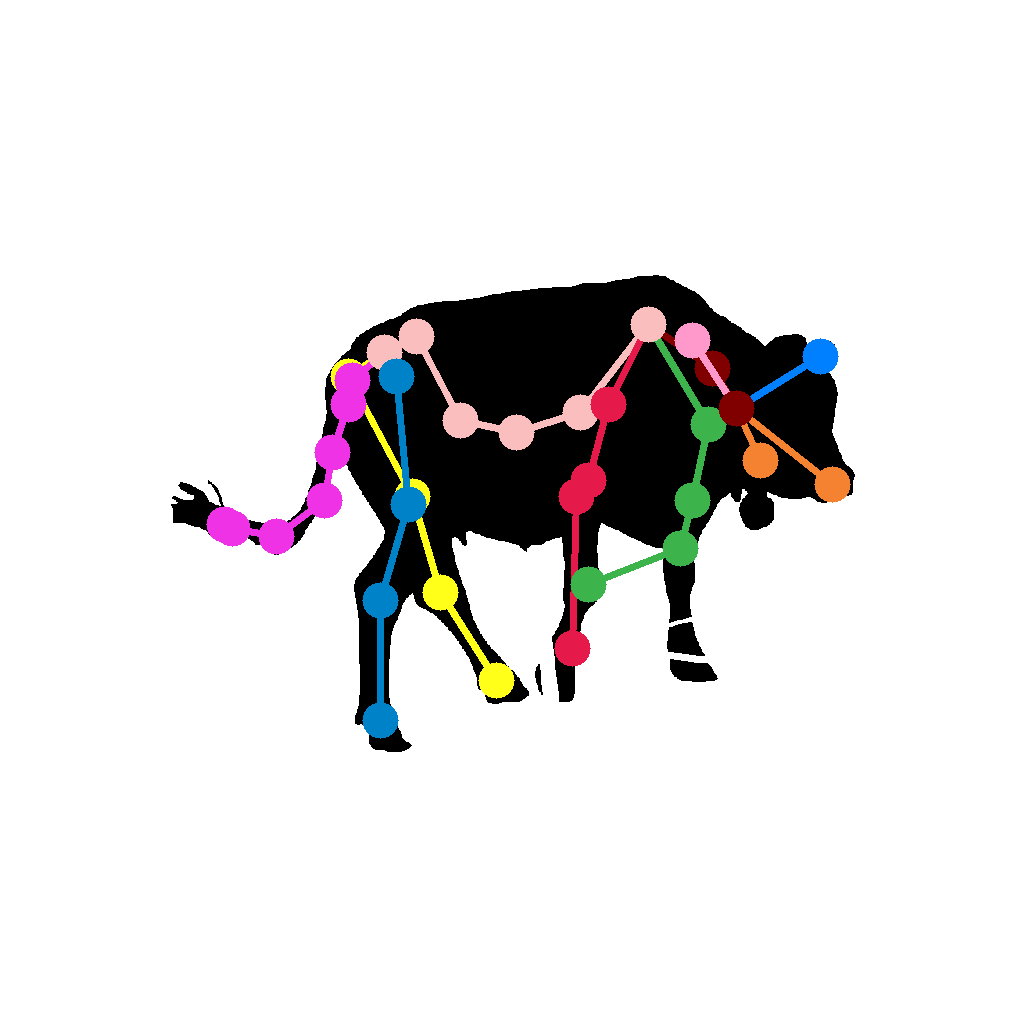
\includegraphics[trim={6cm 6cm 6cm 6cm},clip,height=\comparisonheight]{ga_vs_qp/0069_skel_sil_raw.png}
        &
    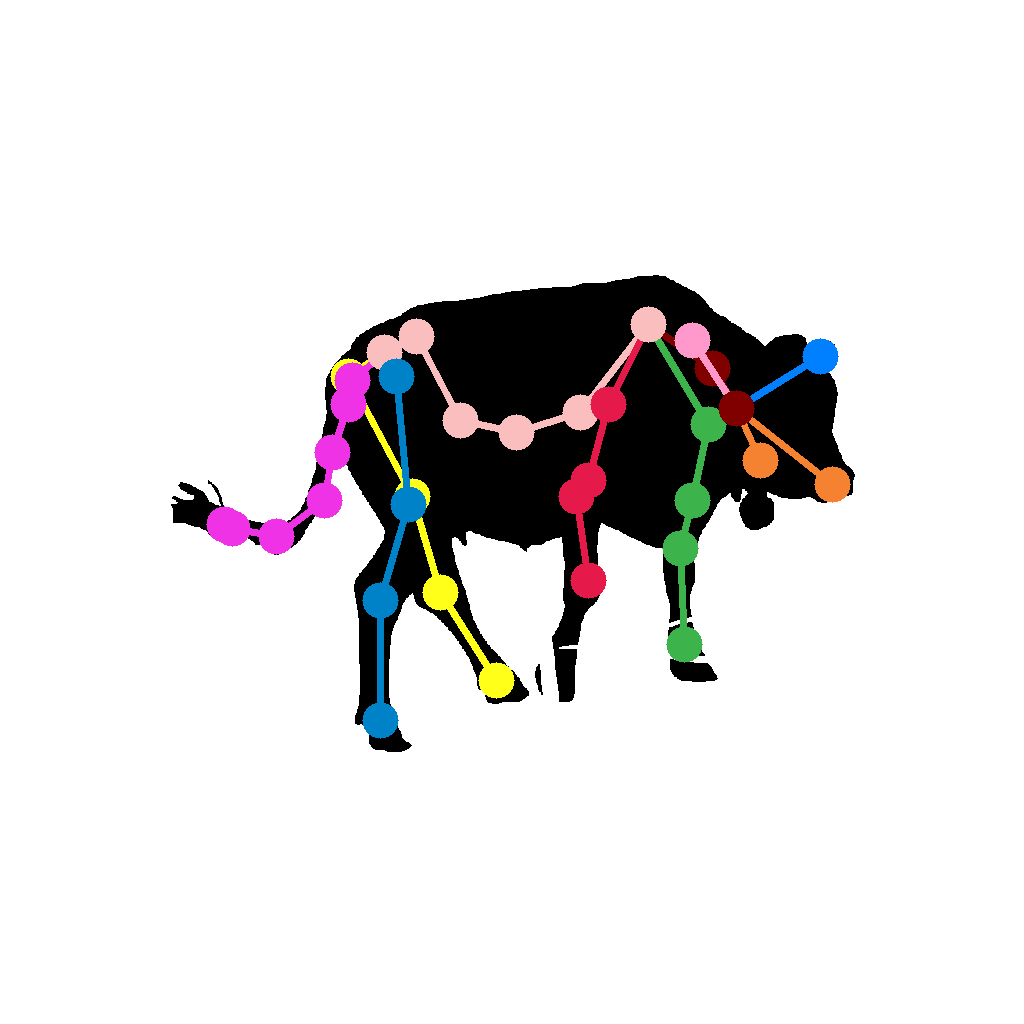
\includegraphics[trim={6cm 6cm 6cm 6cm},clip,height=\comparisonheight]{ga_vs_qp/0069_skel_sil_cleaned_qp.png}
        &
    {}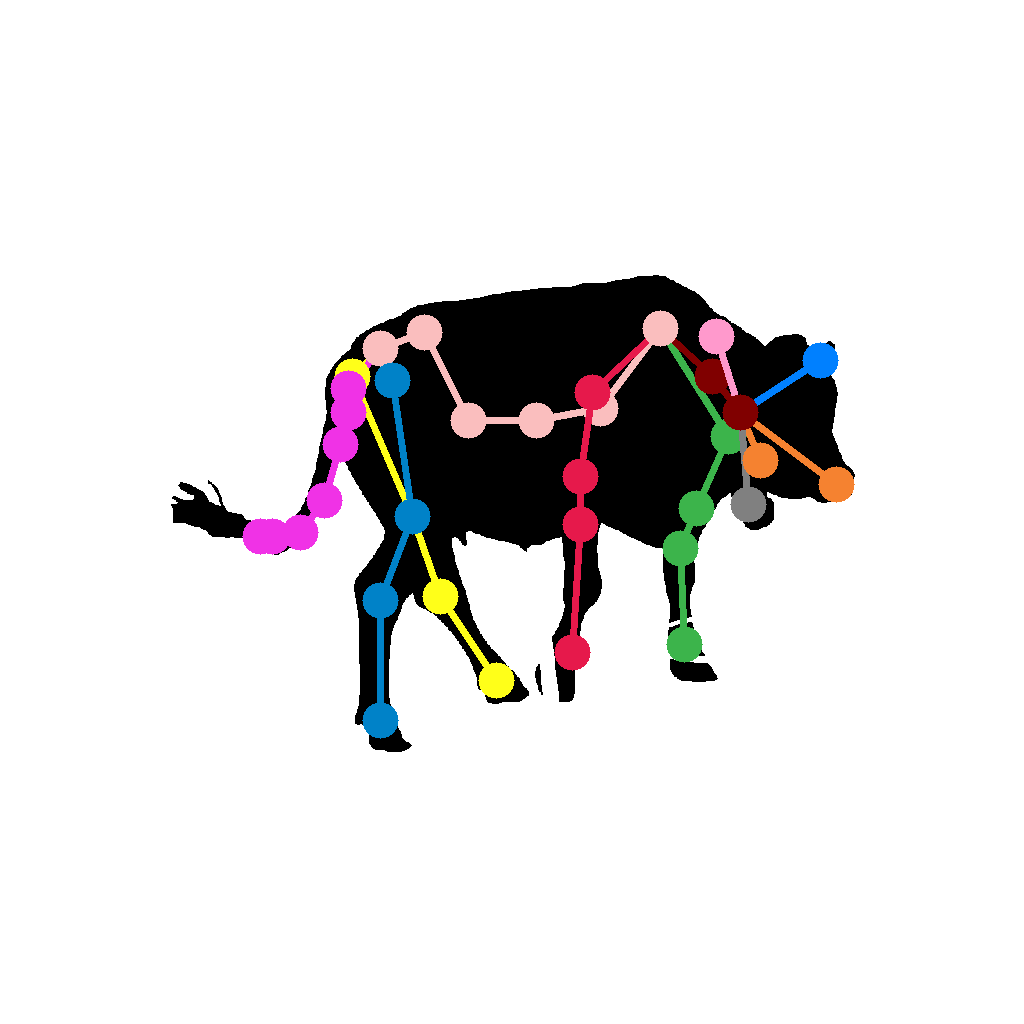
\includegraphics[trim={6cm 6cm 6cm 6cm},clip,height=\comparisonheight]{ga_vs_qp/0069_skel_sil_cleaned_ga.png} \\
    (a) & (b) & (c)
\end{tabular}
}{
\caption{Example skeletons from raw predictions (a), processed with OJA-QP (b), and OJA-GA (c).}
\label{fig:comparison}
}
~
\capbtabbox{%
\small
\begin{tabular}{lccc}
\toprule
                & Raw       & QP        & GA    \\
\midrule
bear           & 83.1      & 83.7      & \textbf{88.9}   \\
camel          & 73.3      & 74.1      & \textbf{87.1}   \\
cat            & 58.5      & \textbf{60.1}      & 58.4    \\
cows           & 89.2      & 88.4      & \textbf{94.7}  \\
dog            & \textbf{66.9}  & 66.6   & \textbf{66.9}  \\
horsejump-high & 26.5      & \textbf{27.7}      & 24.4   \\
horsejump-low  & 26.9      & 27.0      & \textbf{31.9}   \\
tiger          & 76.5      & 88.8      & \textbf{92.3}   \\
rs\_dog        & 64.2      & 63.4      & \textbf{81.2}   \\
\midrule
Average        & 62.8      & 64.4      & \textbf{69.5}   \\
\bottomrule
\end{tabular}
}{\caption{Accuracy of OJA on BADJA test sequences.}
\label{tab:animal}
}
\end{floatrow}
\end{figure}

\begin{table}[ht]
\centering
\small
\begin{tabular}{@{}cccccccccc@{}}

\toprule
        \multirow{2}{*}{Seq.}  & \multirow{2}{*}{Family} & \multicolumn{2}{c}{PCK (\%)} &   \multirow{2}{*}{Mesh}  & \multirow{2}{*}{Seq.} & \multirow{2}{*}{Family} & \multicolumn{2}{c}{PCK (\%)} &   \multirow{2}{*}{Mesh} \\
&  & Raw                  & OJA-GA &  &&& Raw                  & OJA-GA           \\ \midrule
01 & Felidae         & 91.8     & 91.9  & 38.2   &  06 & Equidae         & 84.4     & 84.8  & 19.2     \\
02 & Felidae         & 94.7     & 95.0  & 42.4   &  07 & Bovidae         & 94.6     & 95.0  & 40.6     \\
03 & Canidae         & 87.7     & 88.0  & 27.3   &  08 & Bovidae        & 85.2     & 85.8  & 41.5     \\  
04 & Canidae         & 87.1     & 87.4  & 22.9   &  09 & Hippopotamidae  & 90.5     & 90.6  & 11.8     \\
05 & Equidae         & 88.9     & 89.8  & 51.6   &  10 & Hippopotamidae  & 93.7     & 93.9  & 23.8     \\    
\bottomrule
\end{tabular}%

\caption{Quantitative evaluation on synthetic test sequences. The performance of the raw network outputs and OJA methods are evaluated using the probability of correct keypoint (PCK) metric. Mesh fitting accuracy is evaluated by computing the mean distance between the predicted and ground truth vertices.}
\label{tab:synthetic}
\end{table}


\begin{figure}[t]
\def\bb{\rule{2in}{0pt}\rule{0pt}{1in}}
\def\bjb{\rule{0.5in}{0pt}\rule{0pt}{0.25in}}
\setlength{\fboxsep}{0pt}%
\centering
\begin{tabular}{ccc}
\includegraphics[width=0.3\linewidth]{smal_comp_cat/rgb_cropped.jpg}
&
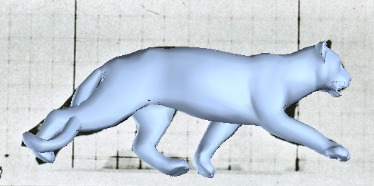
\includegraphics[width=0.3\linewidth]{smal_comp_cat/muybridge_107_smal_res_cropped.jpg}
&
\includegraphics[width=0.3\linewidth]{smal_comp_cat/3d_fit_overlay_rgb_cropped.jpg}
\\

\includegraphics[width=0.3\linewidth]{smal_comp_horse/rgb_cropped.jpg} &
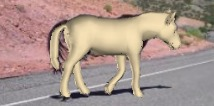
\includegraphics[width=0.3\linewidth]{smal_comp_horse/00049424_ferrari_smal_cropped.jpg} &

\includegraphics[width=0.3\linewidth]{smal_comp_horse/3d_fit_overlay_rgb_cropped.jpg} \\

RGB & SMAL \cite{zuffi2017menagerie} & \textbf{Ours}
\end{tabular}
\caption{Results are comparable in quality to SMAL~\cite{zuffi2017menagerie}, but note that we do not require hand-clicked keypoints.
}
\label{fig:compar_smal}
\end{figure}
    

\subsection{Model fitting}
The predicted joint positions and silhouette are input to the 3D model fitting optimization phase, which proceeds in four stages. The first stage solves for the model's global rotation and translation parameters, which positions the camera. Following SMPLify~\cite{bogo16keep}, this camera stage is solved for torso points only, which remain largely fixed through shape and pose variation. The remaining stages solve for all shape, pose and translation parameters the emphasis of the priors gradually decreased. The silhouette term is introduced in the penultimate stage, as including this too early can lead to the optimizer finding unsatisfactory local minima.

The final outputs of our optimization pipeline are shown in \figref{example_results}. In each of the cases illustrated the optimizer is able to successfully find a set of pose and shape parameters which, when rendered, closely resembles the input image. The final row of \figref{example_results} demonstrates the generalizability of the proposed method: the algorithm is able to find a reasonable pose despite no camel figurines being included in the original SMAL model.

\subsubsection*{Comparison to other work.} Our approach is compared visually to that given by Zuffi {\em et al.}~\cite{zuffi2017menagerie}. Recall that their results require hand-clicked keypoints rather than fitting to points predicted automatically by the hourglass network, which was trained on synthetic animal images. Further, their work is optimized for single frame fitting and is tested on animals in simple poses, whereas the focus of this work is on the more challenging task of tracking animals in video. \figref{compar_smal} shows the application of our model to a number of single frame examples from the SMAL result data~\cite{zuffi2017menagerie}.

\subsubsection*{Quantitative experiments.}
There is no existing ground truth dataset for comparing reconstructed 3D animal meshes, but an estimate of quantitative error is obtained by testing on synthetic sequences for a range of quadruped species. These are generated by randomly deforming the model and varying the camera position to animate animal motion, see Figure~\ref{fig:synth}. Table~\ref{tab:synthetic} shows results on these sequences. 
%bjb_insert

\begin{figure}[t!]
\begin{tabular}{cccccc}
\includegraphics[width=0.16\linewidth]{synth_pipeline_45/gt_fit_cropped.png} & 
\includegraphics[width=0.16\linewidth]{synth_pipeline_45/3d_fit_cropped.png} &

\includegraphics[width=0.16\linewidth]{synth_pipeline_50/gt_fit_cropped.png} &
\includegraphics[width=0.16\linewidth]{synth_pipeline_50/3d_fit_cropped.png} &

\includegraphics[width=0.16\linewidth]{synth_pipeline_55/gt_fit_cropped.png} &
\includegraphics[width=0.16\linewidth]{synth_pipeline_55/3d_fit_cropped.png} \\
\end{tabular}
\caption{Evaluating synthetic data. Green models: ground truth, Orange models: predicted. Frames 5, 10 and 15 of sequence 4 shown. Error on this sequence 22.9.}
\label{fig:synth}
\end{figure}
    

\subsection{Automatic silhouette prediction}
While not the main focus of our work, the system presented in this chapter is able to perform the full 3D reconstruction process from an input image with no user intervention. This is achieved by incorporating the DeepLabv3+ network~\cite{deeplabv3plus} as a front-end segmentation engine which automatically generates animal silhouettes. This network was trained on the PASCAL VOC 2012 dataset, which includes a variety of animal quadruped classes. An example result generated using the fully automatic pipeline is shown in \figref{overview}.


\begin{figure}[h!]
\def\bb{\rule{2in}{0pt}\rule{0pt}{1in}}
\def\lp#1[#2]#3{\parbox{0.16\linewidth}{\labelledpic{#1}{\includegraphics[#2]{#3}}}}
\begin{tabular}{cccccc}
\includegraphics[trim={0 2cm 0 1.25cm},clip,width=0.16\linewidth]{res_bear_new/rgb.jpg} & 

\includegraphics[trim={0 2cm 0 1.25cm},clip,width=0.16\linewidth]{res_bear_new/target.jpg} & 
\includegraphics[trim={0 2cm 0 1.25cm},clip,width=0.16\linewidth]{res_bear_new/heatmap.jpg} & 
\includegraphics[trim={0 2cm 0 1.25cm},clip,width=0.16\linewidth]{res_bear_new/cleaned_skeleton_sil.jpg} &
\includegraphics[trim={0 2cm 0 1.25cm},clip,width=0.16\linewidth]{res_bear_new/3d_fit_overlay_rgb.jpg} & 
\includegraphics[trim={0 2cm 0 1.25cm},clip,width=0.16\linewidth]{res_bear_new/3d_fit_reversed.jpg} \\

\includegraphics[trim={0 0.5cm 0 0.5cm},clip,width=0.16\linewidth]{res_horse_new/rgb.jpg} & 

\includegraphics[trim={0 0.5cm 0 0.5cm},clip,width=0.16\linewidth]{res_horse_new/target.jpg} & 
\includegraphics[trim={0 0.5cm 0 0.5cm},clip,width=0.16\linewidth]{res_horse_new/heatmap.jpg} & 
\includegraphics[trim={0 0.5cm 0 0.5cm},clip,width=0.16\linewidth]{res_horse_new/cleaned_skeleton_sil.jpg} &
\includegraphics[trim={0 0.5cm 0 0.5cm},clip,width=0.16\linewidth]{res_horse_new/3d_fit_overlay_rgb.jpg} & 
\includegraphics[trim={0 0.5cm 0 0.5cm},clip,width=0.16\linewidth]{res_horse_new/3d_fit_reversed.jpg} \\

\includegraphics[trim={0 1.5cm 0 1.5cm},clip,width=0.16\linewidth]{res_rsdog158_new/rgb.jpg} & 

\includegraphics[trim={0 1.5cm 0 1.5cm},clip,width=0.16\linewidth]{res_rsdog158_new/target.jpg} & 
\includegraphics[trim={0 1.5cm 0 1.5cm},clip,width=0.16\linewidth]{res_rsdog158_new/heatmap.jpg} & 
\includegraphics[trim={0 1.5cm 0 1.5cm},clip,width=0.16\linewidth]{res_rsdog158_new/cleaned_skeleton_sil.jpg} &
\includegraphics[trim={0 1.5cm 0 1.5cm},clip,width=0.16\linewidth]{res_rsdog158_new/3d_fit_overlay_rgb.jpg} & 
\includegraphics[trim={0 1.5cm 0 1.5cm},clip,width=0.16\linewidth]{res_rsdog158_new/3d_fit_reversed.jpg} \\

\lp a[trim={0 1cm 0 1cm},clip,width=0.98\linewidth]{res_camel_new/rgb.jpg} & 
\lp b[trim={0 1cm 0 1cm},clip,width=0.98\linewidth]{res_camel_new/target.jpg} & 
\lp c[trim={0 1cm 0 1cm},clip,width=0.98\linewidth]{res_camel_new/heatmap.jpg} & 
\lp d[trim={0 1cm 0 1cm},clip,width=0.98\linewidth]{res_camel_new/cleaned_skeleton_sil.jpg} &
\lp e[trim={0 1cm 0 1cm},clip,width=0.98\linewidth]{res_camel_new/3d_fit_overlay_rgb.jpg} & 
\lp f[trim={0 1cm 0 1cm},clip,width=0.98\linewidth]{res_camel_new/3d_fit_reversed.jpg} 
\end{tabular}
\caption{Example results on various animals. From left to right: RGB input, extracted silhouette, network-predicted heatmaps, OJA-processed joints, overlay 3D fit and alternative view.}
\label{fig:example_results}
\end{figure}

\begin{figure}[h!]
\centering
\def\p#1{\includegraphics[trim={0 1cm 0 1cm},clip,height=0.12\linewidth] {dog_agility_blooper/#1.jpg}}
\p{target}
\p{3d_fit_overlay_rgb}
\def\p#1{\includegraphics[trim={0 1cm 0 1cm},clip,height=0.12\linewidth] {elephant_blooper/#1.jpg}}
\p{target}
\p{3d_fit_overlay_rgb}
\def\p#1{\includegraphics[trim={0 1cm 0 1cm},clip,height=0.12\linewidth] {rhino_blooper/#1.jpg}}
\p{target}
\p{3d_fit_overlay_rgb}

\caption{Failure modes of the proposed system. \emph{Left}: Missing interior contours prevent the optimizer from identifying which way the dog is facing. \emph{Middle}: The model has never seen an elephant, so assumes the trunk is the tail. \emph{Right}: Heavy occlusion. The model interprets the tree as background and hence the silhouette term tries to minimize coverage over this region.}
\label{fig:blooper}
\end{figure}
\section{Conclusions}
The chapter introduces a technique for reconstructing 3D quadrupeds from video by using a quadruped model parameterized in shape and pose. By incorporating automatic segmentation tools, the pipeline can be deployed without requiring human intervention or even precise knowledge of the species of animal being considered. The method performs well on examples encountered in the real world, generalizes to unseen animal species and is robust to challenging shapes and poses. 

As a direction for future work, it would be worthwhile to look at methods for synthetic image generation that preserve important edge information lost during silhouette extraction. In particular, the lost interior contours cause ambiguities which necessitate the OJA method described here. An alternative is to extend the recent work of SMALST~\lazycite{SMALST}{SMALST} (which requires hand-clicked training images) by instead synthetizing realistic textures using generative adverserial networks. Of course, it is important to ensure the texture generation process preserves the sampled pose parameters. A naive method is to rendering texture as a UV map on top of the SMAL model, but this could also be framed as an image-to-image translation problem, beginning with a low detail SMAL render and mapping to a photorealistic image with a carefully designed pose-preserving generator. Other components of the system which could be improved would be building a more sophisticated motion prior, able to represent likely animal trajectories. In addition, robustness to environmental factors as shown in \Cref{fig:blooper} could be improved by rendering synthetic causes of occlusion (perhaps even as rectangles). 
    